\documentclass[11pt,a4paper]{article}
\usepackage[margin=0.8in]{geometry}
\usepackage{setspace}
\usepackage{booktabs}
\usepackage{array}
\usepackage{longtable}
\usepackage{titlesec}
\usepackage{url}
\usepackage[colorlinks=true,linkcolor=blue,urlcolor=blue,citecolor=blue]{hyperref}
\usepackage{graphicx}
\usepackage{float}
\usepackage{caption}
\titleformat{\section}{\large\bfseries}{\thesection.}{0.5em}{}
\titleformat{\subsection}{\normalsize\bfseries}{\thesubsection.}{0.5em}{}
\setstretch{1.05}
\renewcommand{\arraystretch}{0.95}
\captionsetup{font=footnotesize}
\setlength{\textfloatsep}{8pt}
\setlength{\floatsep}{6pt}
\setlength{\intextsep}{6pt}

\begin{document}

\begin{center}
{\LARGE Smart Document Parser: Resume Entity Extraction}\\[6pt]
{\large Project Report (Assignment 3)}\\[6pt]
{\normalsize GitHub Repo: \href{https://github.com/Akshat-A-K/Resumer-Parser}{https://github.com/Akshat-A-K/Resumer-Parser}}\\[4pt]
{\normalsize Team: Akshat Kotadia (2025201005, akshat.kotadia@students.iiit.ac.in)\\
Om Mehra (2025201008, om.mehra@students.iiit.ac.in)\\
Ankit Chavda (2025201045, chavda.ankitbhai@students.iiit.ac.in)}
\end{center}

\section{Abstract}
We built a resume parser that converts PDF or image resumes into clean JSON. The system uses OCR and PDF text extraction, and a local LLM (Ollama with Llama 3.2) to extract entities like name, email, skills, education, and experience. A Streamlit web app lets the user upload a file, review the output, edit it, and download the final JSON. We also created an evaluation mode that compares predictions with a labeled dataset and reports precision, recall, and F1 scores. This report explains the problem, dataset, method, and results for two approaches. The code is in the branches: ollama-basic and prompt-based-fine-tuning. Both branches are considered in this submission.


\section{Introduction}
In hiring, companies receive many resumes for one job opening. Manually reading each resume and writing the details is slow. So we need an automated system that can read a resume and extract important data in a structured format. The assignment asks for a smart document parser, and we selected the resume parsing task. Our system is fully local and works without paid APIs.

\section{Problem Statement and Objectives}
The system should take a resume in PDF or image form and return a structured JSON with key information. It should handle different layouts and noisy text and still give usable results.

We allow both PDF resumes and image resumes (PNG, JPG, JPEG, BMP, TIFF, WEBP). For images we use OCR, and for PDFs we extract text directly.

Main objectives:
\begin{itemize}
\item Extract contact, education, experience, skills, and projects.
\item Provide a simple UI for upload, review, edit, and download.
\item Provide evaluation results on labeled data.
\end{itemize}

\section{Dataset}
We used the Resume Entities for NER dataset from Kaggle \cite{dataset}. It has 220 annotated resume samples in newline-delimited JSON format. Each sample has resume text and labeled entity spans. The labeled fields include Name, Email Address, Location, Designation, Companies worked at, Skills, College Name, Degree, Graduation Year, and Years of Experience. Many fields in our schema (such as phone, links, projects, or certifications) do not have ground truth in the dataset, so evaluation is only for the mapped 10 fields.

\section{Approach 1: Streamlit Application (ollama-basic)}
This approach is in the branch ollama-basic. The pipeline is:
\begin{enumerate}
\item User uploads a PDF or image.
\item Text is extracted using PDF parsers for PDF, and OCR for images.
\item A strict JSON schema prompt is sent to the local LLM.
\item The output is cleaned and validated into the schema.
\item Results are shown in the UI, user can edit, and then download JSON or CSV.
\end{enumerate}

How the Streamlit app looks and how it is used for ML work: the interface is simple and clean, with a left sidebar to choose the mode (Parse One Resume or Evaluate Quality). In the main area, the user sees the file upload, the extracted text preview, and the editable output. For ML work, it is useful because it gives fast feedback, lets us correct output, and makes it easy to test many samples without extra scripts.

Key points of this approach:
\begin{itemize}
\item Uses local Ollama with Llama 3.2 model and temperature 0.
\item Uses a single prompt with selected fields.
\item Results are validated so empty or missing values are handled safely.
\item Evaluation mode runs on a chosen number of labeled samples.
\end{itemize}

\section{Models and Tools Used}
\begin{itemize}
\item Streamlit for the UI \cite{streamlit}.
\item PyMuPDF with pypdf fallback for PDF text extraction \cite{pymupdf}.
\item EasyOCR with Pillow and NumPy for image text extraction \cite{easyocr}.
\item Ollama for local LLM inference (Llama 3.2, model must be downloaded) \cite{ollama,llama32}.
\item Pydantic for schema validation and normalization \cite{pydantic}.
\item Pandas for evaluation tables.
\end{itemize}

\section{Approach 2: Prompt-Based Fine-Tuning (prompt-based-fine-tuning)}
This approach is in the branch prompt-based-fine-tuning. It focuses on stronger prompt engineering and structured extraction. We include it here for comparison.

Key ideas:
\begin{itemize}
\item Section-wise prompting: resume text is split into sections like education, experience, projects, and skills. Each section is parsed with only relevant fields.
\item Extended schema: structured lists are used for education, experience, and projects.
\item Extra normalization: JSON repair, retries, and link mapping to improve output quality.
\item Caching: repeated extractions are faster.
\end{itemize}

This method aims to improve list-heavy fields by reducing prompt noise and focusing on relevant text for each section.

\section{Branch Comparison and Key Differences}
\begin{itemize}
\item prompt-based-fine-tuning has section-wise prompting and stronger JSON repair with retries.
\item It adds a more detailed schema with structured lists for education, experience, and projects.
\item It uses caching to speed up repeated extractions.
\item ollama-basic is simpler and faster, with a single prompt for selected fields.
\item Evaluation scripts and results are organized a bit differently in the two branches.
\end{itemize}

\section{Evaluation Methodology}
We used the labeled dataset to measure accuracy. For string fields, we compute exact match, fuzzy match, and token-based precision/recall/F1. For list fields, we use set-based precision/recall/F1 with fuzzy matching and Jaccard similarity. We also report macro-averaged precision, recall, and F1 across all fields.

\section{Results for Streamlit Approach (10 Samples)}
Latest evaluation for the ollama-basic branch was run on 10 samples. Macro scores:
\begin{itemize}
\item Precision: 0.5712
\item Recall: 0.5883
\item F1: 0.5561
\end{itemize}

\begin{longtable}{p{4cm}cccc}
\toprule
Entity Type & Precision & Recall & F1 & Support \\
\midrule
Name & 0.90 & 0.90 & 0.90 & 9 \\
Graduation Year & 0.40 & 0.40 & 0.40 & 7 \\
Years of Experience & 0.50 & 0.50 & 0.50 & 2 \\
Email & 0.70 & 0.60 & 0.6333 & 8 \\
Location & 0.45 & 0.80 & 0.5633 & 8 \\
Degree & 0.80 & 0.625 & 0.6857 & 8 \\
Designation & 0.70 & 0.65 & 0.6667 & 8 \\
Companies Worked At & 0.2417 & 0.50 & 0.3067 & 8 \\
Skills & 0.15 & 0.20 & 0.1667 & 10 \\
College Name & 0.87 & 0.7083 & 0.7389 & 10 \\
\bottomrule
\end{longtable}

\newpage

\section{Results for Prompt-Based Fine-Tuning Branch (10 Samples)}
Reported macro scores from the prompt-based-fine-tuning branch:
\begin{itemize}
\item Precision: 0.585
\item Recall: 0.617
\item F1: 0.575
\end{itemize}

\begin{longtable}{p{4cm}cccc}
\toprule
Entity Type & Precision & Recall & F1 & Support \\
\midrule
Name & 0.900 & 0.900 & 0.900 & 9 \\
Email & 0.700 & 0.600 & 0.633 & 8 \\
Location & 0.500 & 0.900 & 0.630 & 8 \\
Graduation Year & 0.400 & 0.400 & 0.400 & 7 \\
Years of Experience & 0.600 & 0.550 & 0.566 & 2 \\
College Name & 0.783 & 0.725 & 0.745 & 10 \\
Degree & 0.800 & 0.650 & 0.700 & 8 \\
Designation & 0.600 & 0.583 & 0.550 & 8 \\
Companies Worked At & 0.541 & 0.766 & 0.586 & 8 \\
Skills & 0.028 & 0.100 & 0.044 & 10 \\
\bottomrule
\end{longtable}

\section{Comparison and Discussion}
Macro-average comparison (10 samples each):
\begin{center}
\begin{tabular}{lccc}
\toprule
Approach & Precision & Recall & F1 \\
\midrule
ollama-basic & 0.5712 & 0.5883 & 0.5561 \\
prompt-based-fine-tuning & 0.5850 & 0.6170 & 0.5750 \\
\bottomrule
\end{tabular}
\end{center}

Observations in simple words:
\begin{itemize}
\item Both approaches are strong in name and education fields.
\item The prompt-based branch gives slightly higher macro scores.
\item Prompt-based method takes more time because it runs more steps and more prompts.
\item Skills and companies are the hardest fields in both approaches.
\item Section-wise prompting helps in some list fields, but skills are still weak because of different naming styles.
\end{itemize}

\section{Limitations}
\begin{itemize}
\item The evaluation used only 10 samples, so results can change with more data.
\item OCR quality depends on resume image quality.
\item Some fields are not in the dataset, so they are not evaluated.
\end{itemize}

\section{Conclusion and Future Work}
We built a working resume parser with a Streamlit app, and we also tested a prompt-based fine-tuning approach. The ollama-basic approach is simpler and stable. The prompt-based-fine-tuning approach gives slightly better macro scores on the same sample size, but takes more time. For future work, we should run larger evaluations, improve skill normalization, and try a larger model for better accuracy.

\section{Screenshots}
All screenshots below are from the prompt-based fine-tuning implementation.

\begin{figure}[H]
\centering
\begin{minipage}{0.48\textwidth}
\centering
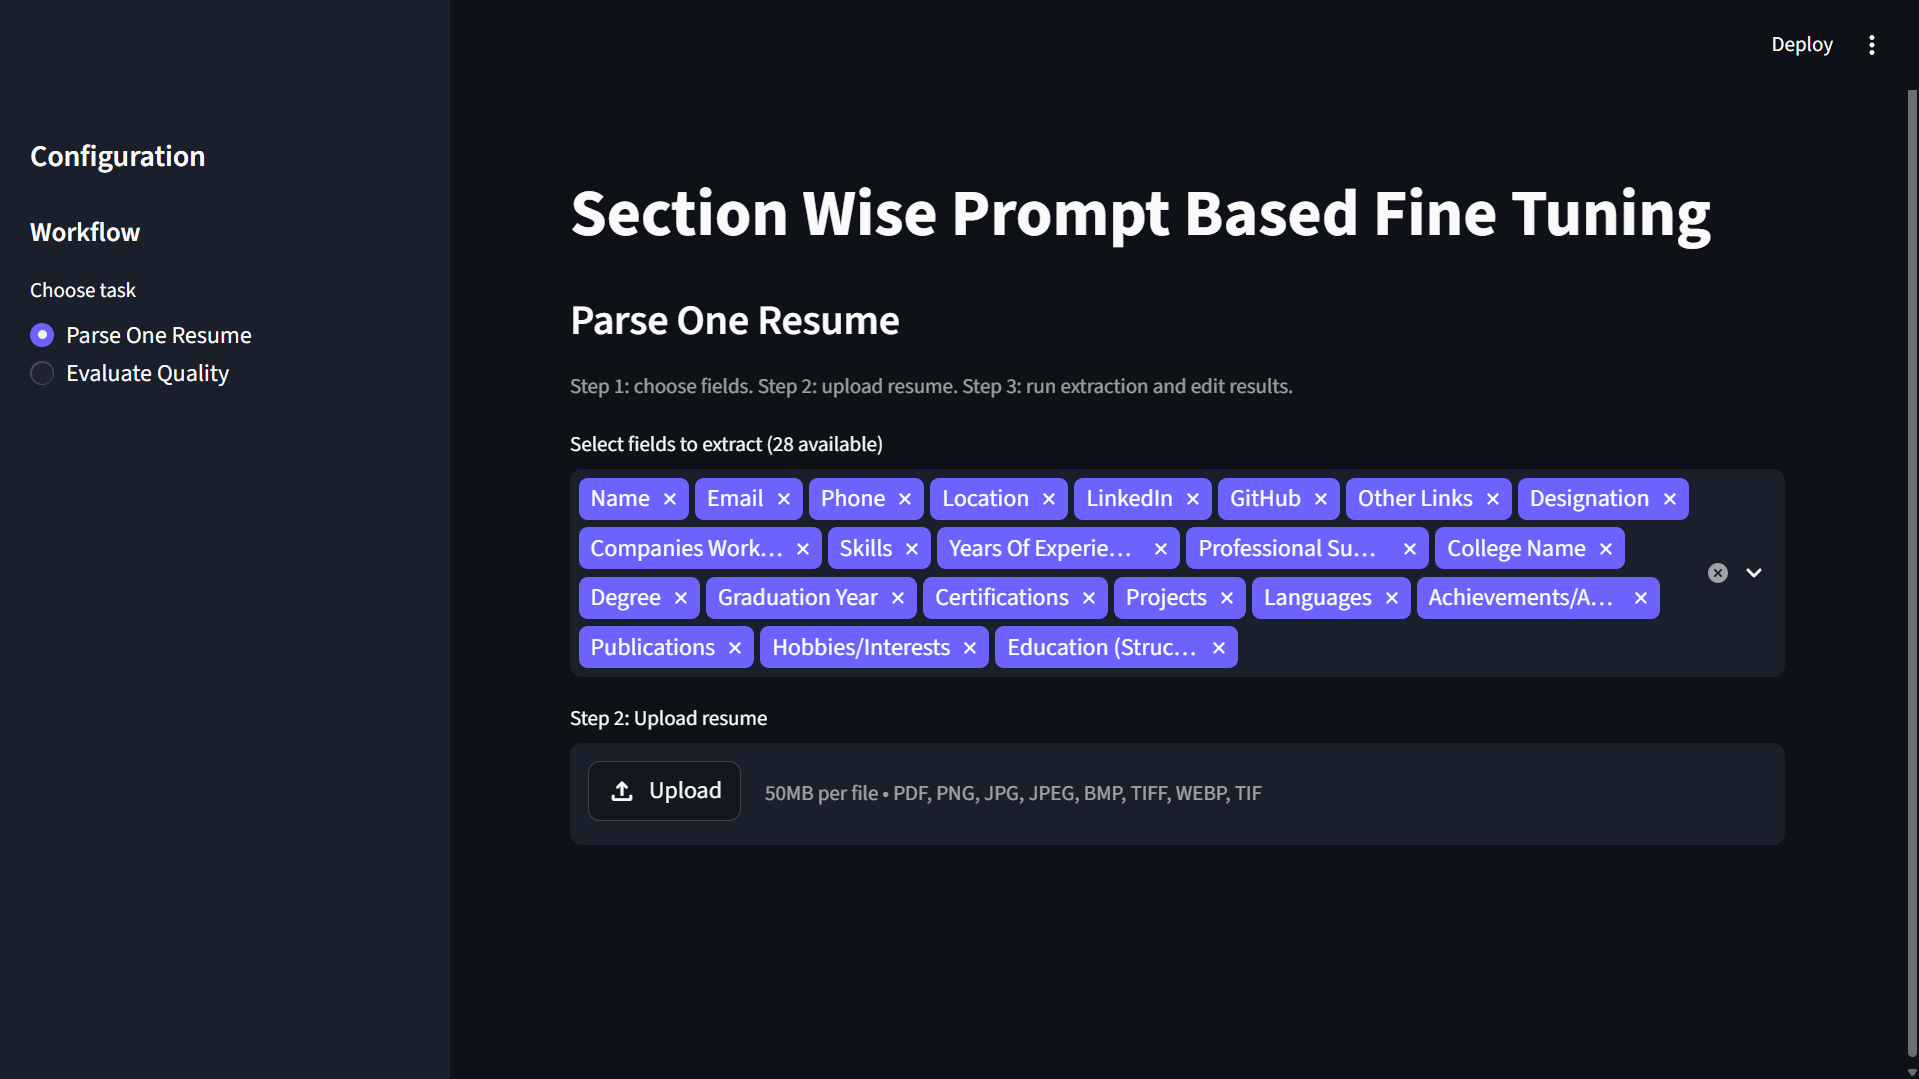
\includegraphics[width=\textwidth]{image4.png}
\\[2pt]
\footnotesize Parse One Resume: field selection and upload
\end{minipage}
\hfill
\begin{minipage}{0.48\textwidth}
\centering
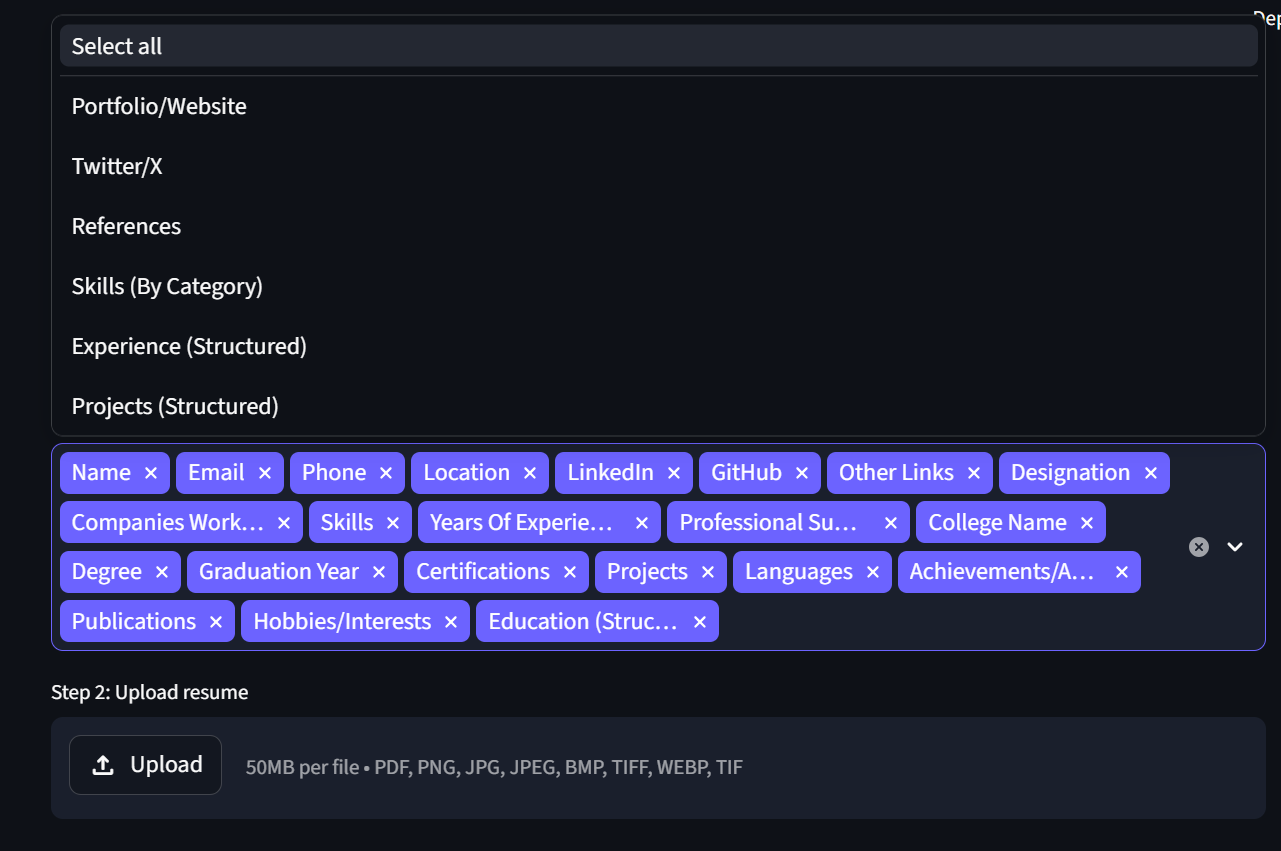
\includegraphics[width=\textwidth]{image5.png}
\\[2pt]
\footnotesize Parse One Resume: field selector dropdown
\end{minipage}
\end{figure}

\begin{figure}[H]
\centering
\begin{minipage}{0.48\textwidth}
\centering
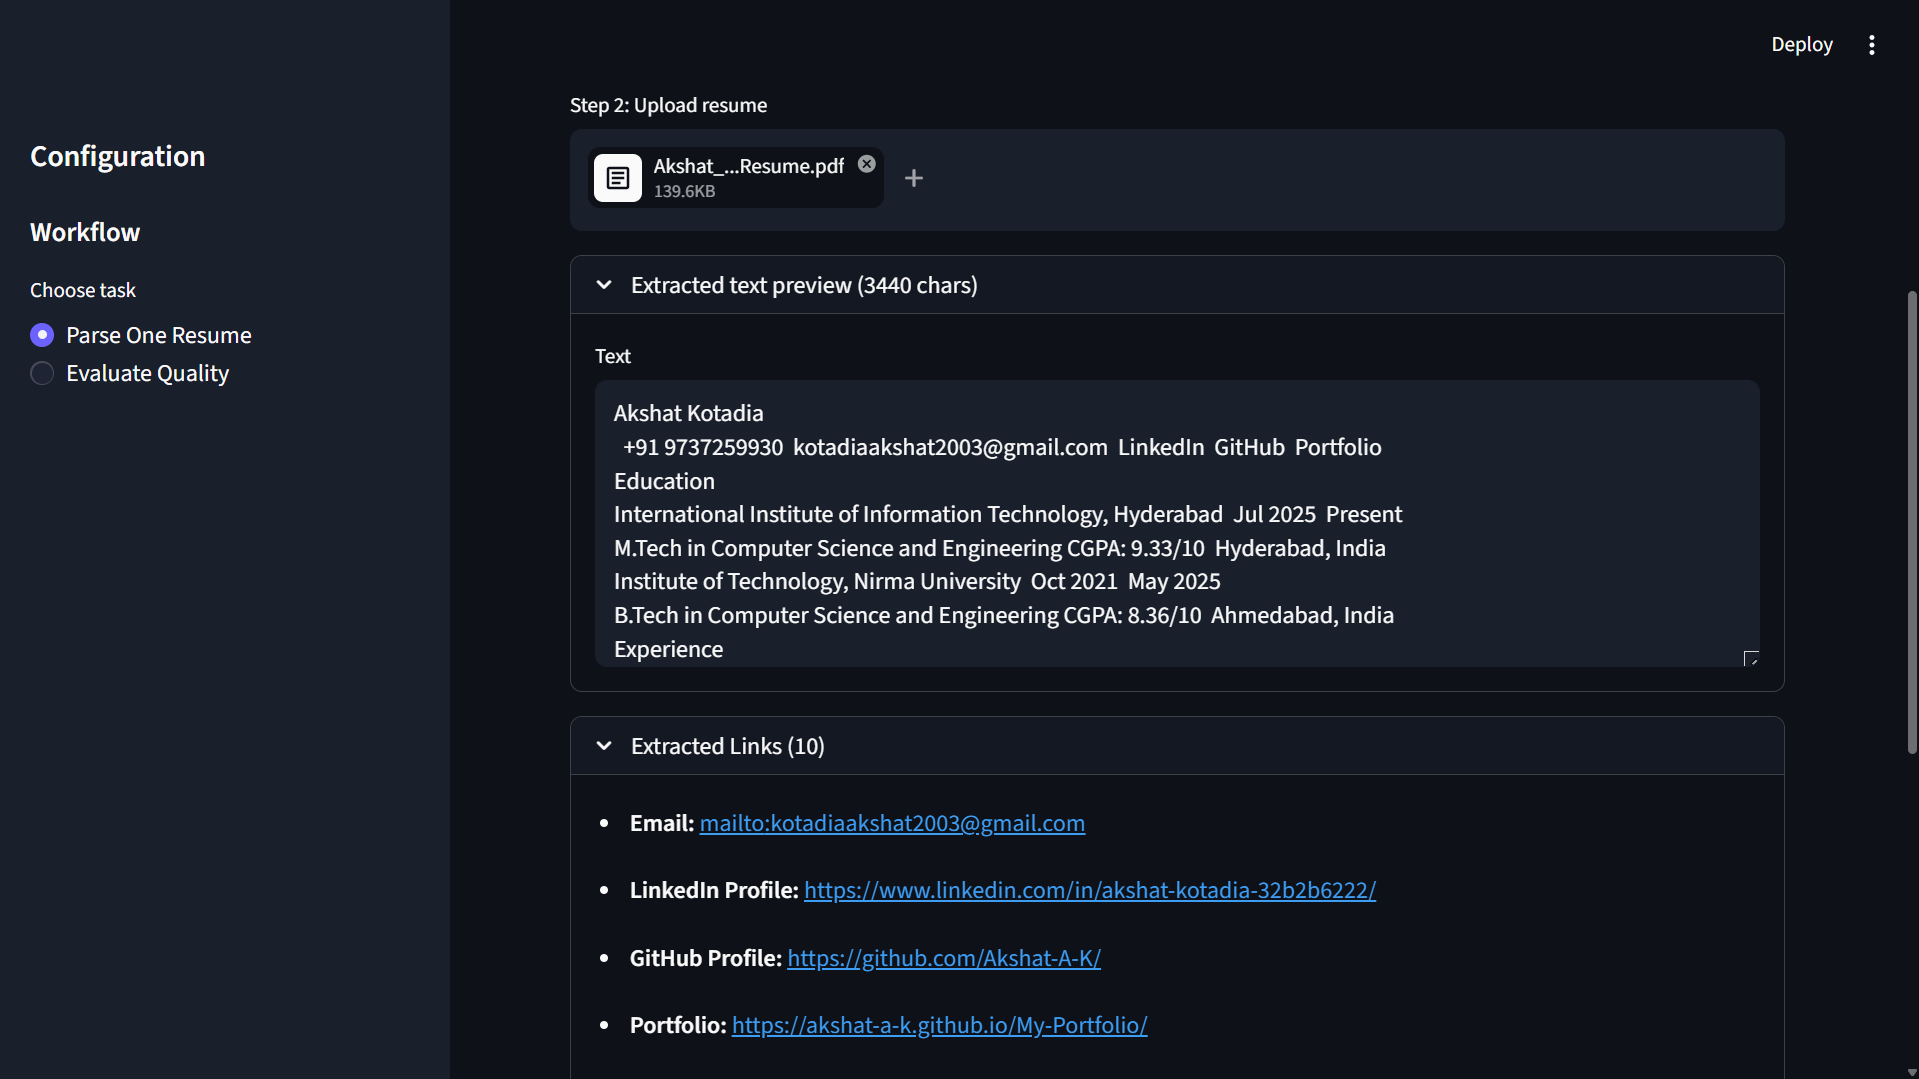
\includegraphics[width=\textwidth]{image6.png}
\\[2pt]
\footnotesize Parse One Resume: extracted text and links preview
\end{minipage}
\hfill
\begin{minipage}{0.48\textwidth}
\centering
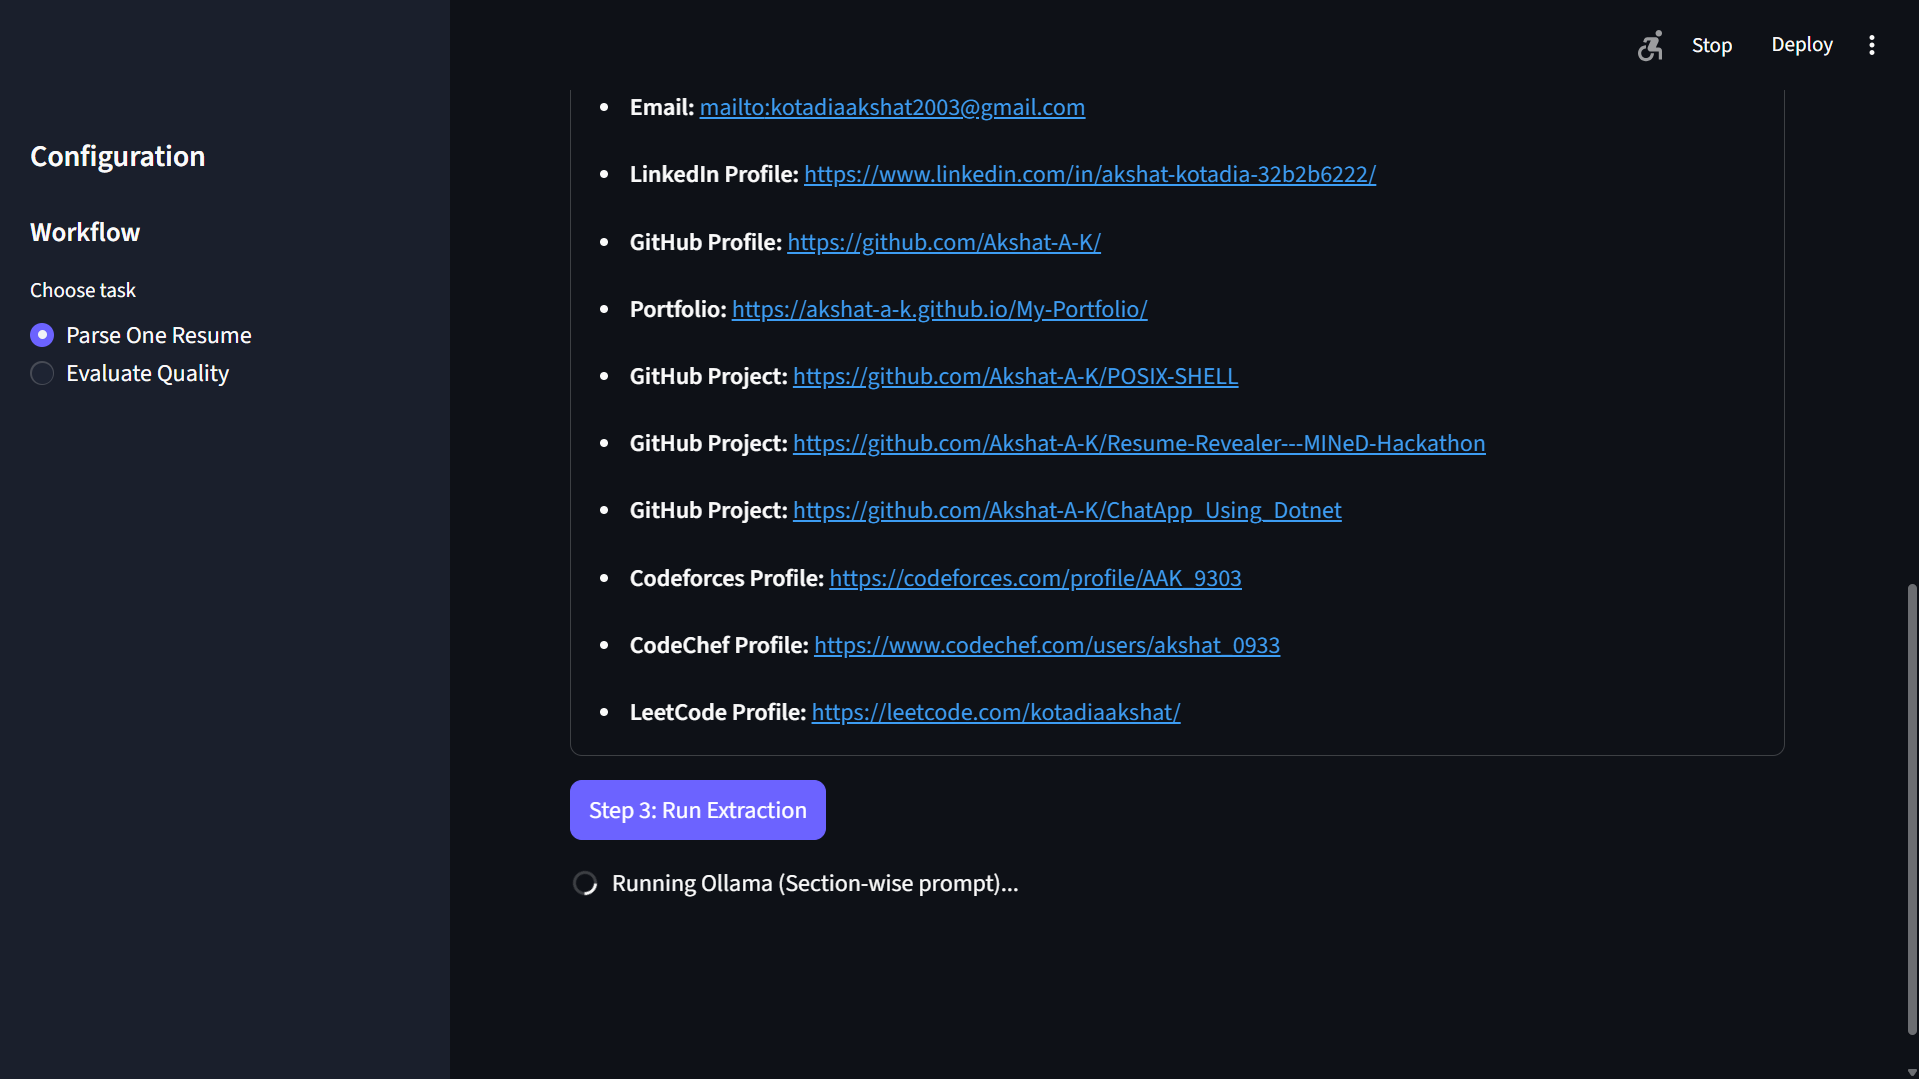
\includegraphics[width=\textwidth]{image7.png}
\\[2pt]
\footnotesize Parse One Resume: run extraction and status
\end{minipage}
\end{figure}

\begin{figure}[H]
\centering
\begin{minipage}{0.48\textwidth}
\centering
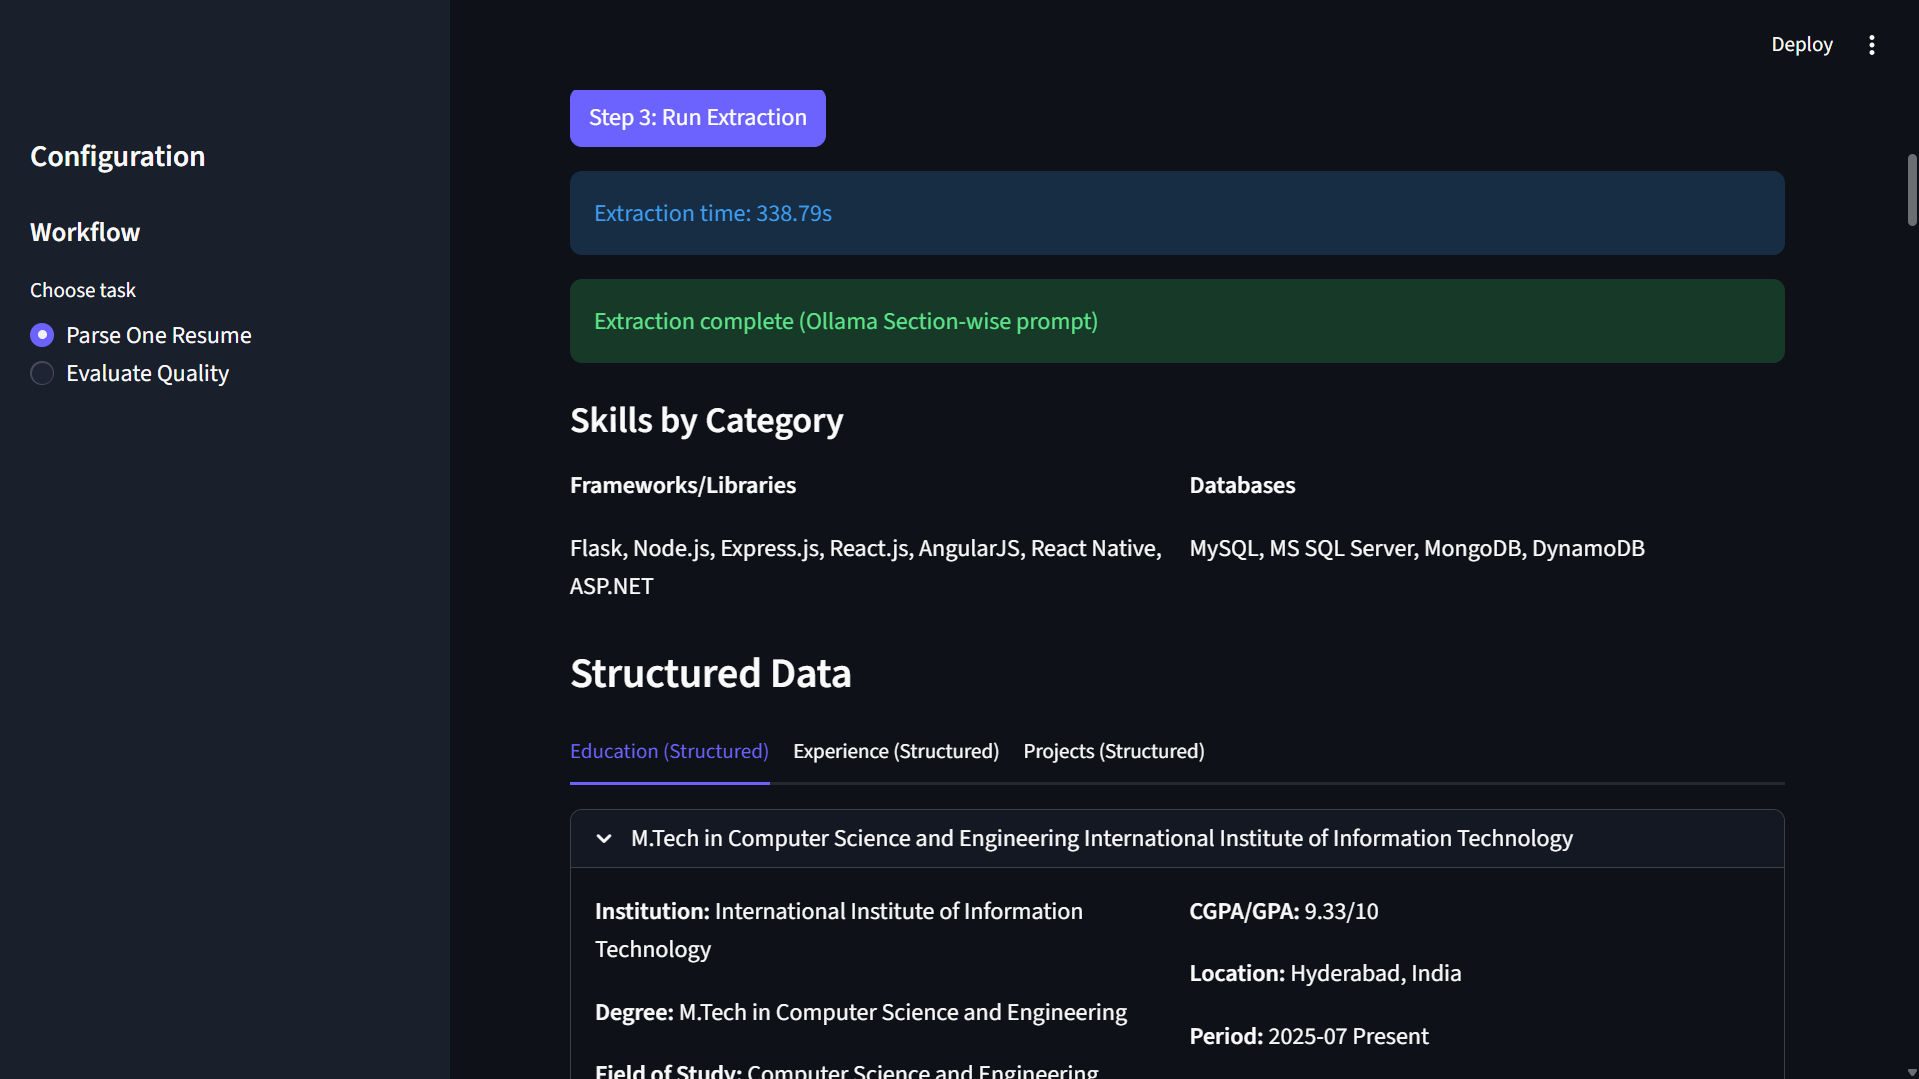
\includegraphics[width=\textwidth]{image8.png}
\\[2pt]
\footnotesize Extraction complete: skills by category and tabs
\end{minipage}
\hfill
\begin{minipage}{0.48\textwidth}
\centering
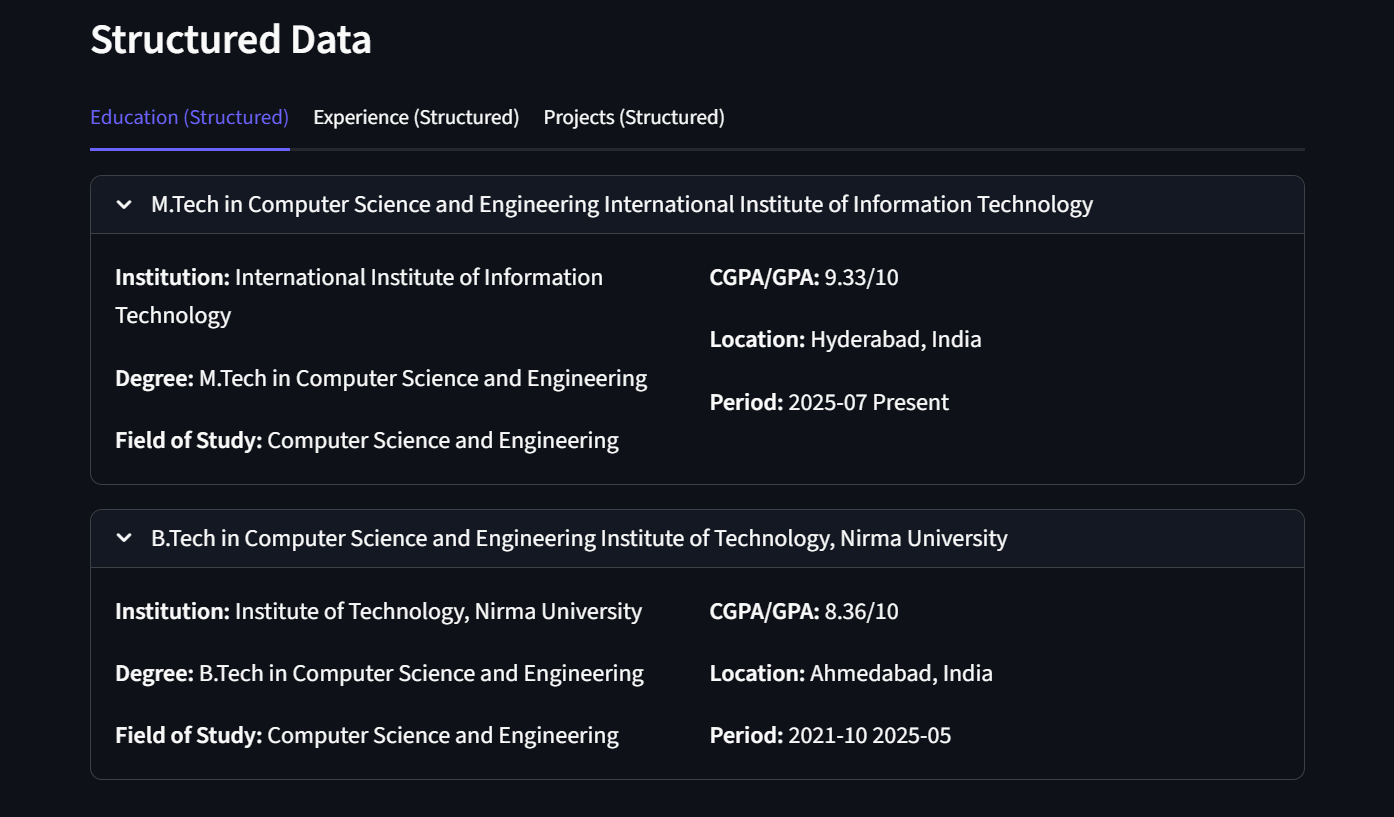
\includegraphics[width=\textwidth]{image9.png}
\\[2pt]
\footnotesize Structured Data: education tab
\end{minipage}
\end{figure}

\begin{figure}[H]
\centering
\begin{minipage}{0.48\textwidth}
\centering
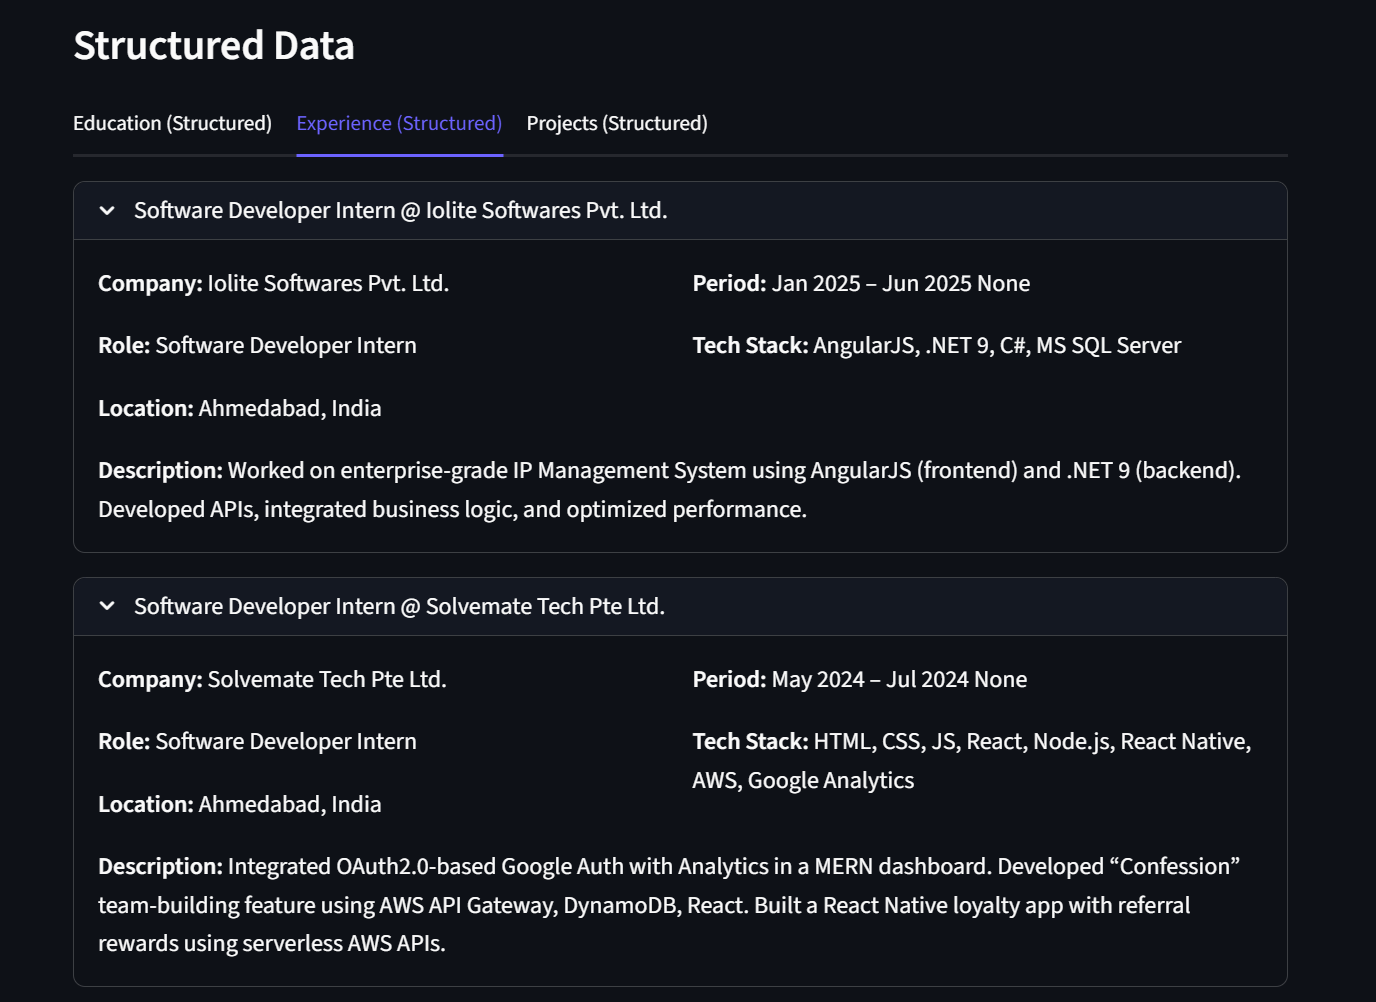
\includegraphics[width=\textwidth]{image10.png}
\\[2pt]
\footnotesize Structured Data: experience tab
\end{minipage}
\hfill
\begin{minipage}{0.48\textwidth}
\centering
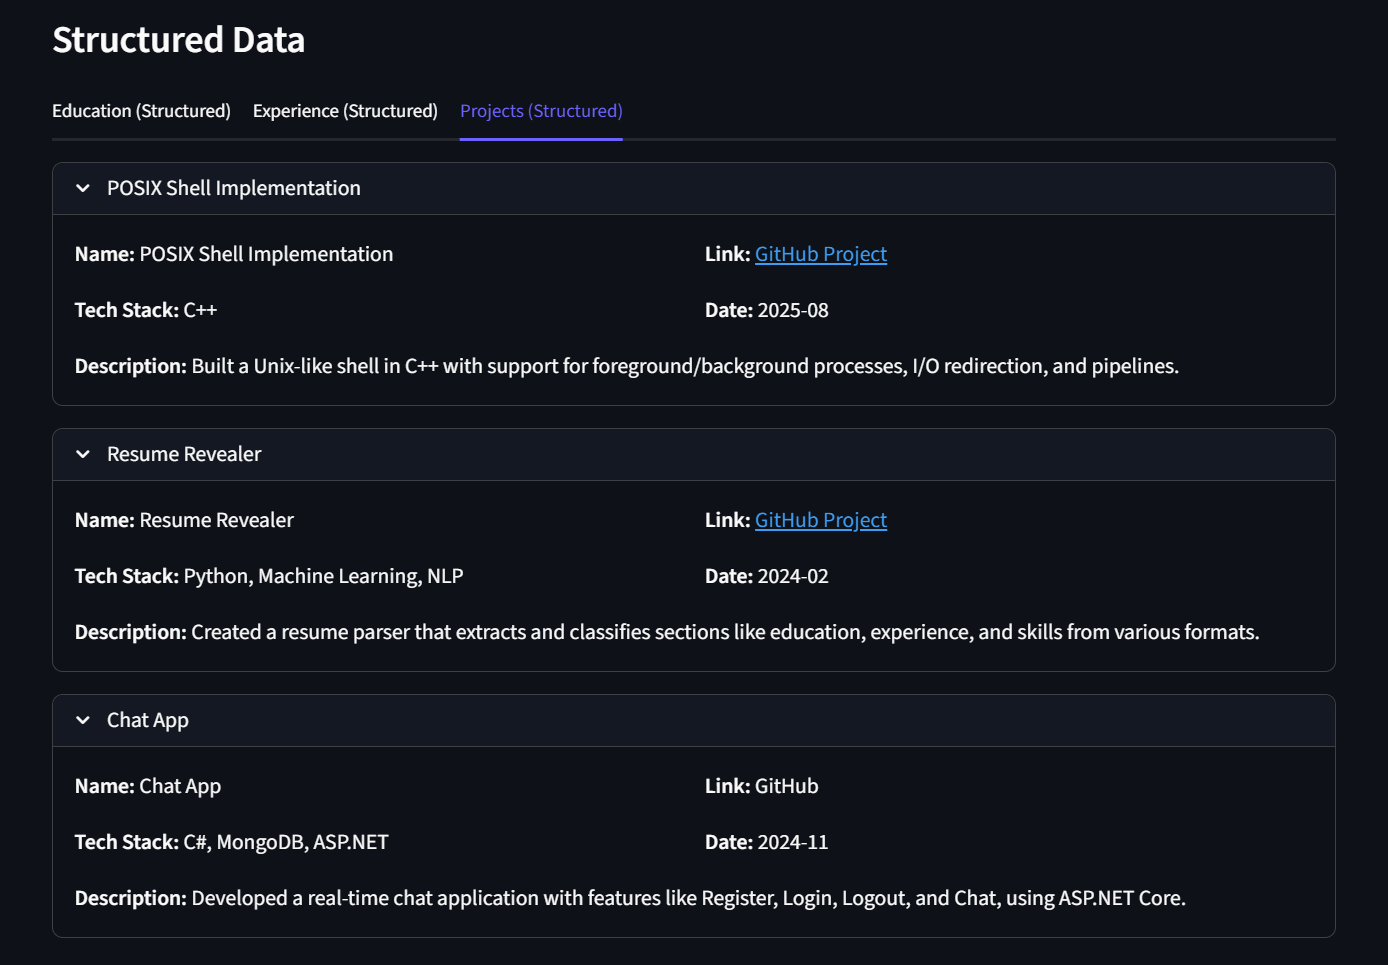
\includegraphics[width=\textwidth]{image11.png}
\\[2pt]
\footnotesize Structured Data: projects tab
\end{minipage}
\end{figure}

\begin{figure}[H]
\centering
\begin{minipage}{0.48\textwidth}
\centering
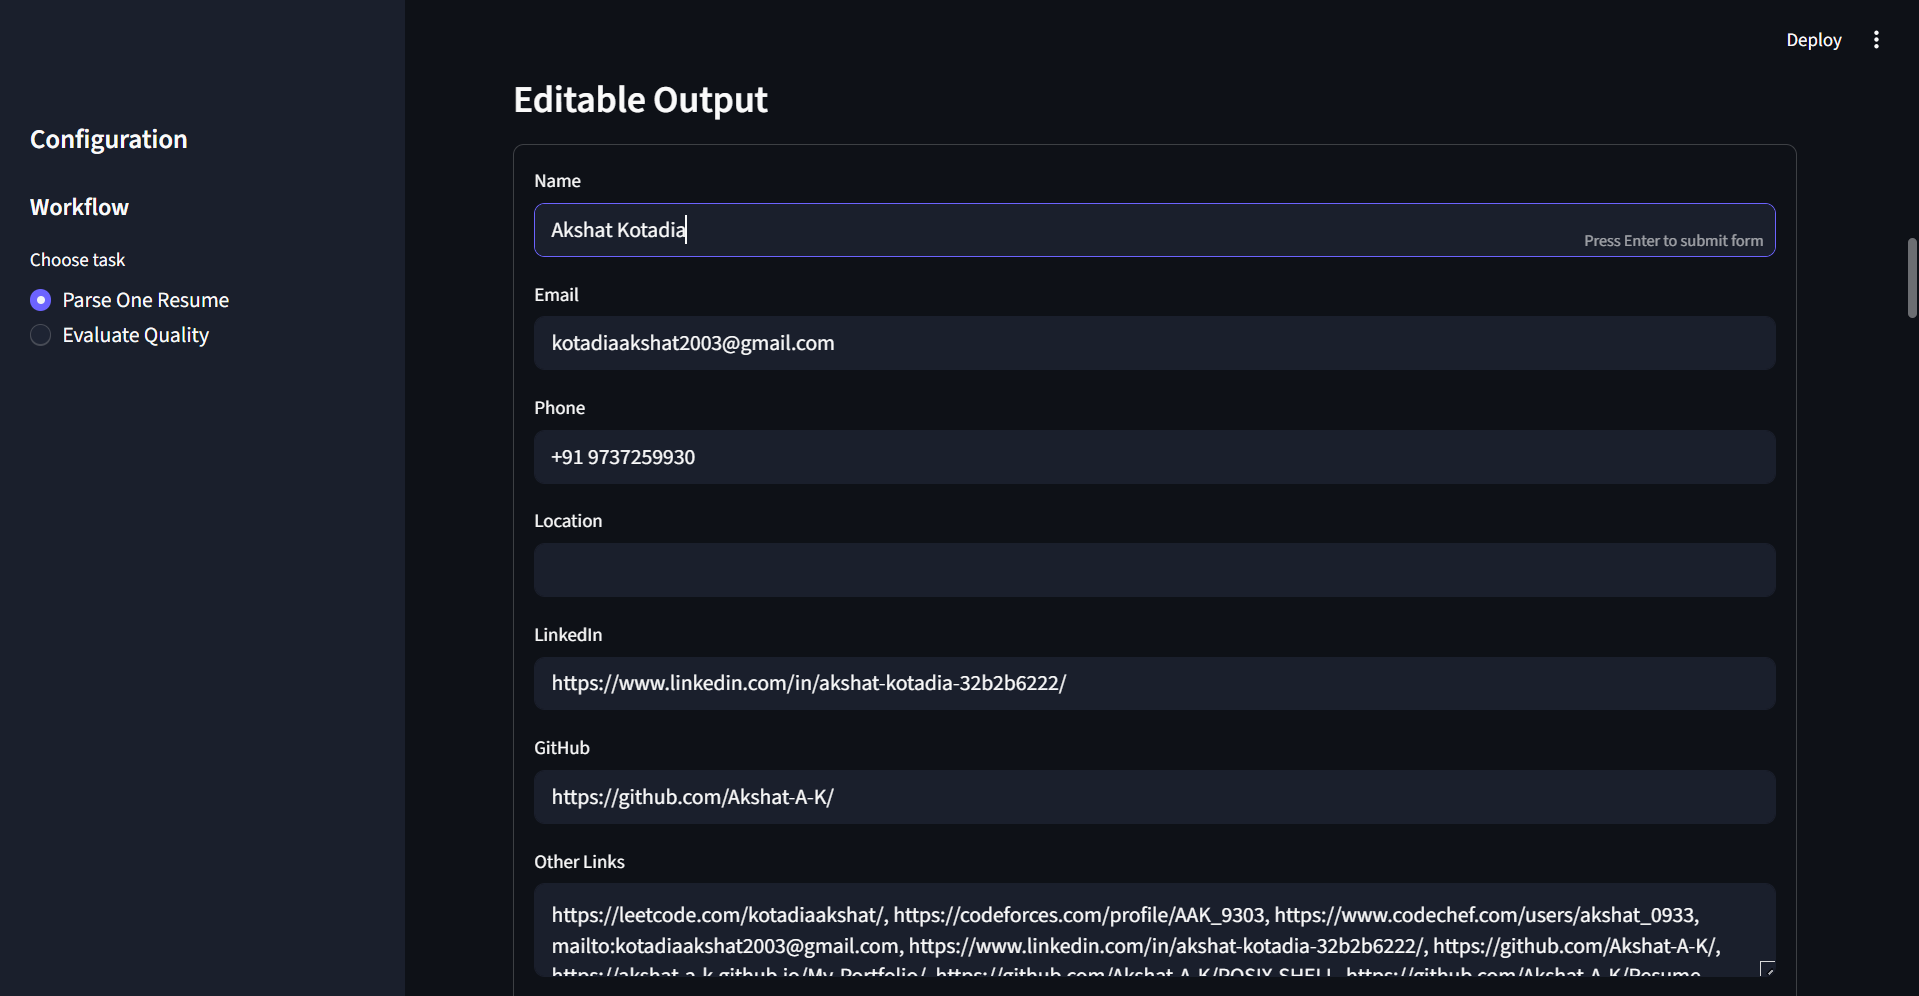
\includegraphics[width=\textwidth]{image12.png}
\\[2pt]
\footnotesize Editable output: basic fields
\end{minipage}
\hfill
\begin{minipage}{0.48\textwidth}
\centering

\includegraphics[width=\textwidth]{image13.png}
\\[2pt]
\footnotesize Editable output: work and skills fields
\end{minipage}
\end{figure}

\begin{figure}[H]
\centering
\begin{minipage}{0.48\textwidth}
\centering
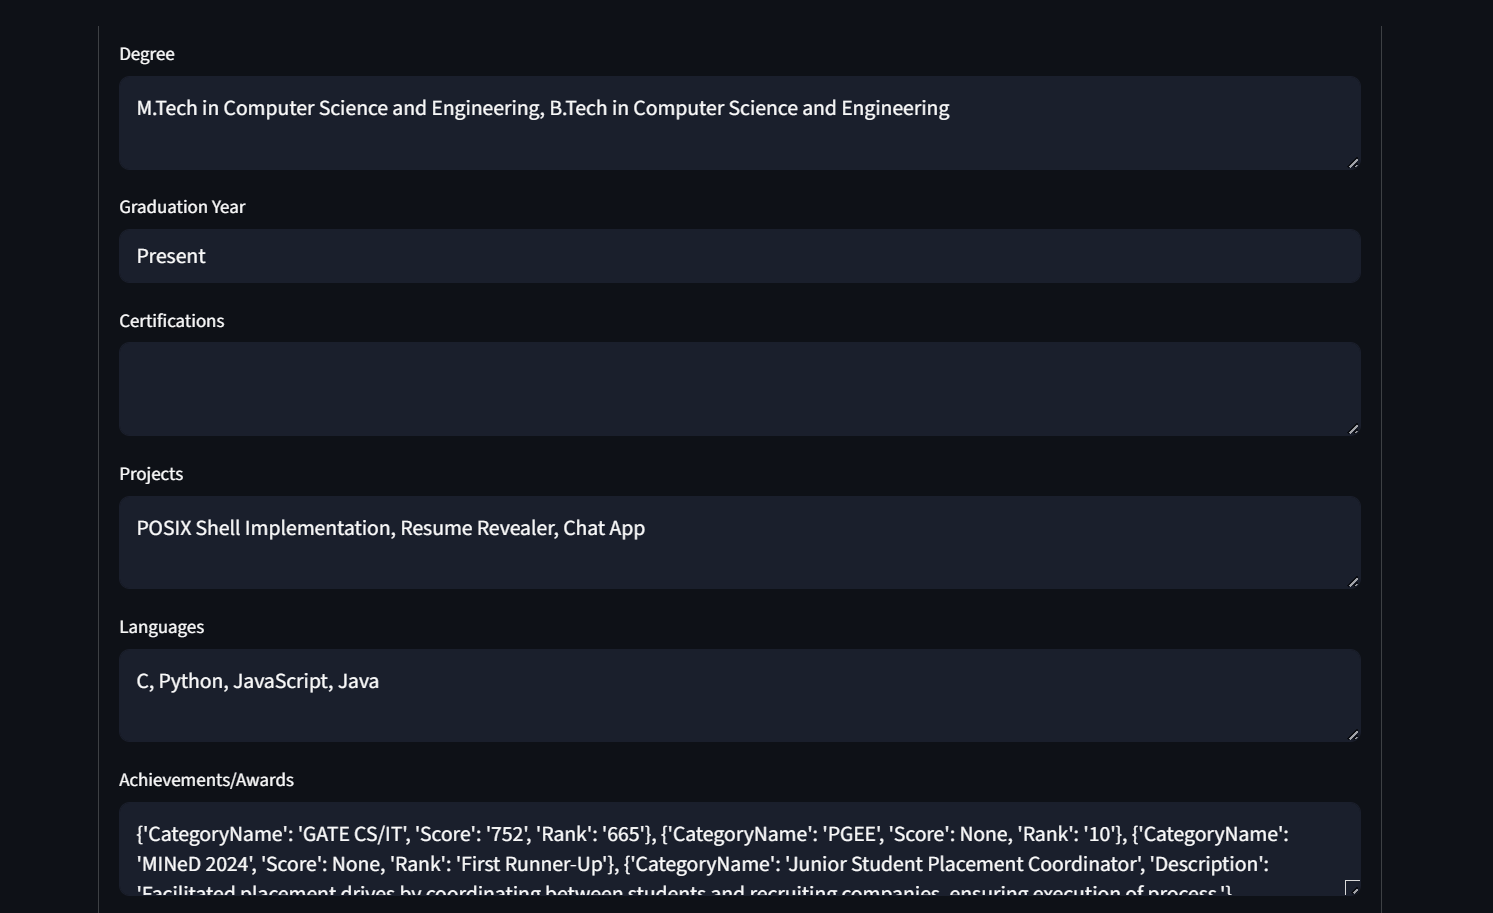
\includegraphics[width=\textwidth]{image14.png}
\\[2pt]
\footnotesize Editable output: projects, languages, achievements
\end{minipage}
\hfill
\begin{minipage}{0.48\textwidth}
\centering
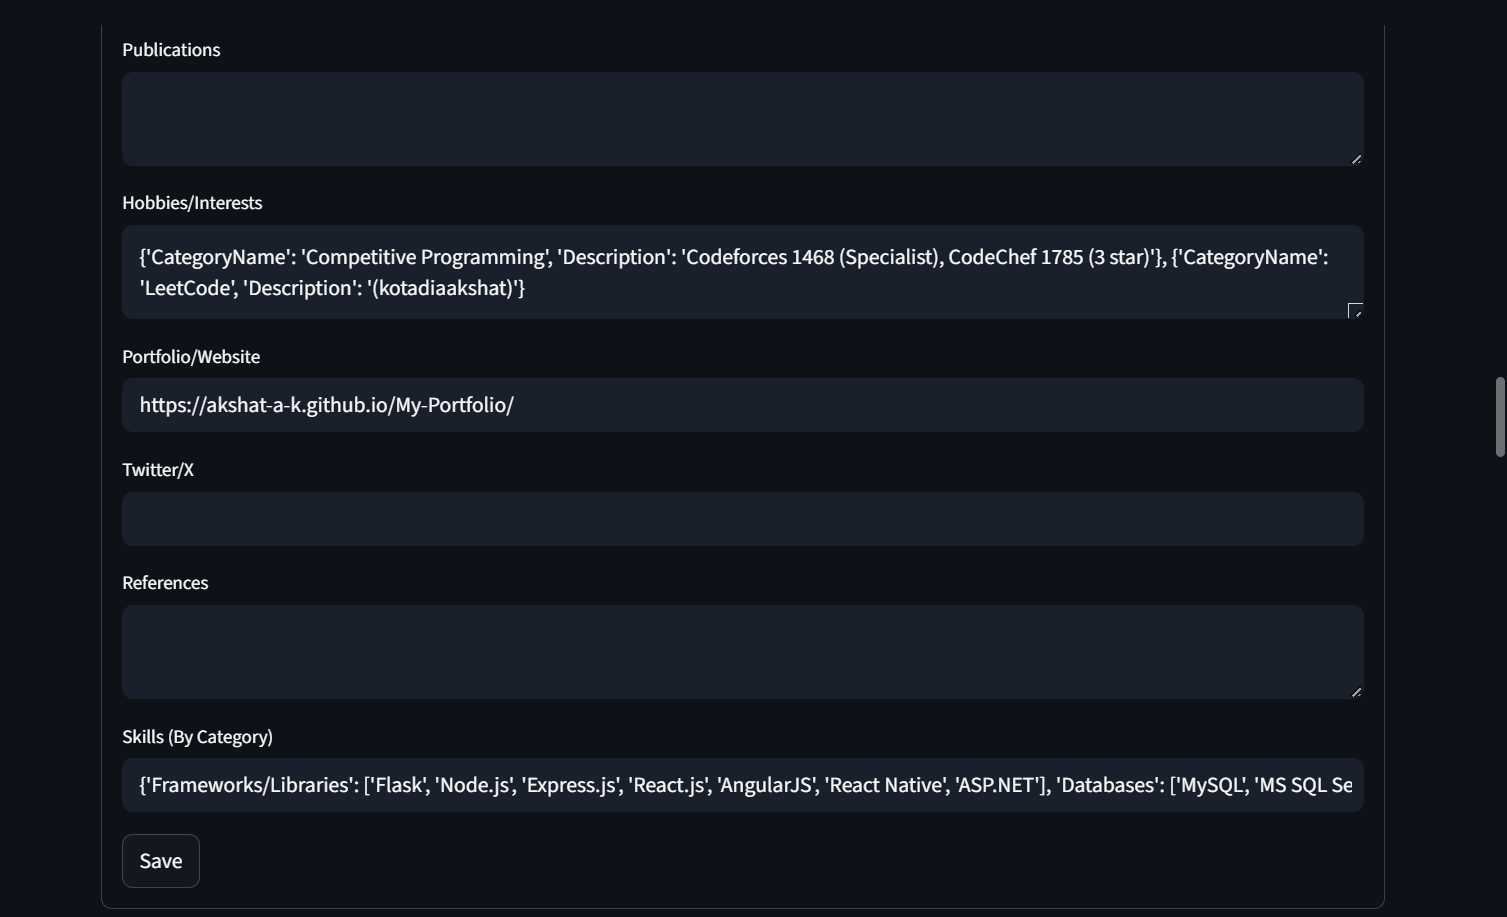
\includegraphics[width=\textwidth]{image15.png}
\\[2pt]
\footnotesize Editable output: publications, hobbies, skills by category
\end{minipage}
\end{figure}

\begin{figure}[H]
\centering
\begin{minipage}{0.48\textwidth}
\centering
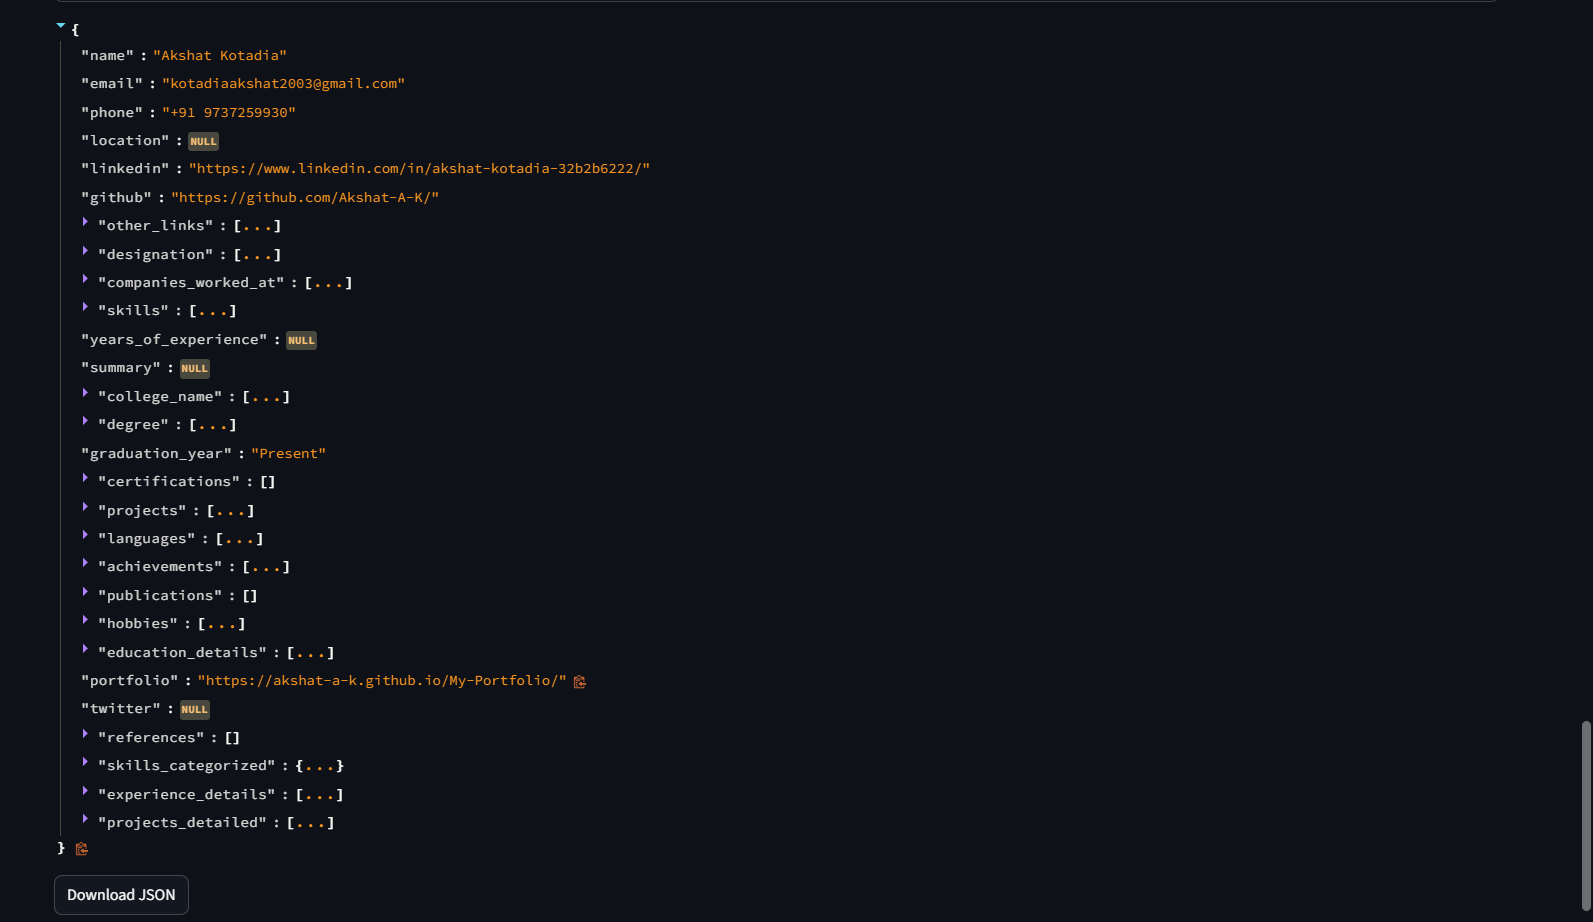
\includegraphics[width=\textwidth]{image16.png}
\\[2pt]
\footnotesize Final JSON output view and download
\end{minipage}
\hfill
\begin{minipage}{0.48\textwidth}
\centering
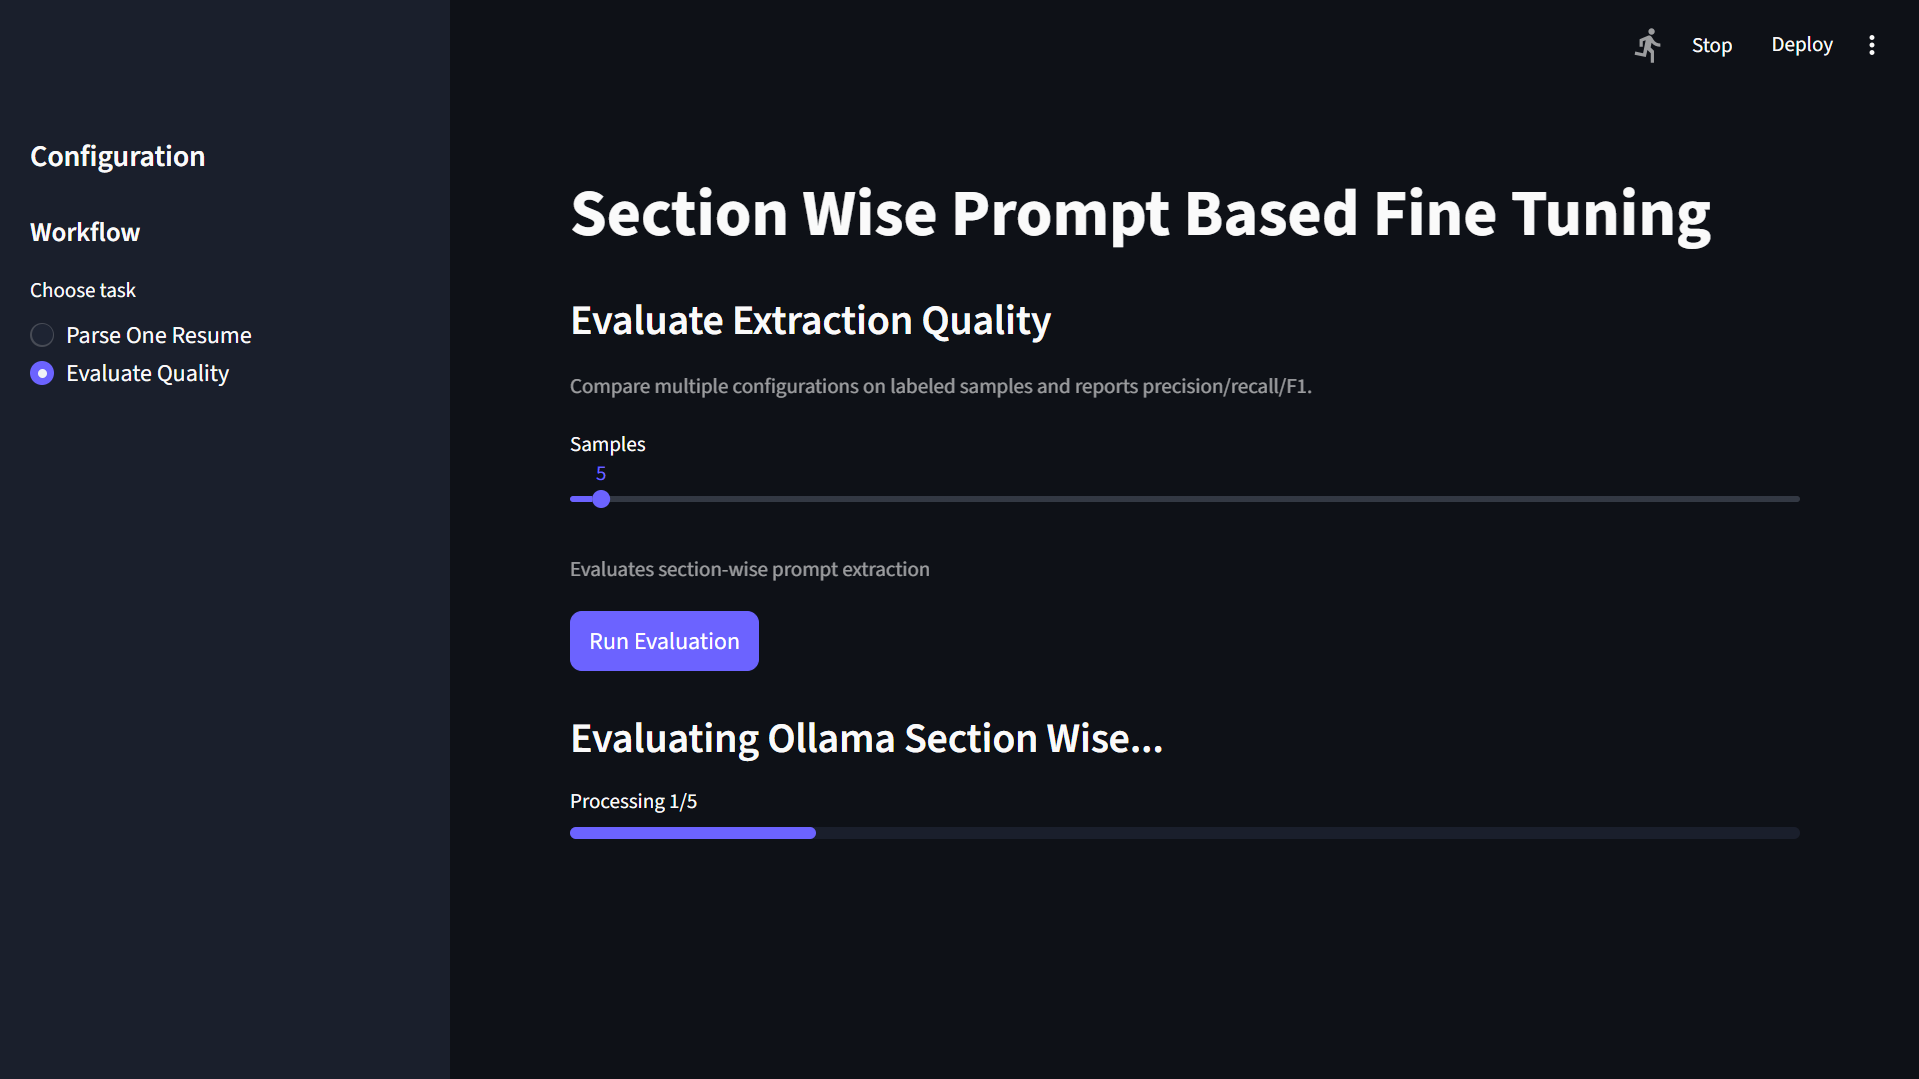
\includegraphics[width=\textwidth]{image17.png}
\\[2pt]
\footnotesize Evaluate Quality: run setup and progress
\end{minipage}
\end{figure}

\begin{figure}[H]
\centering
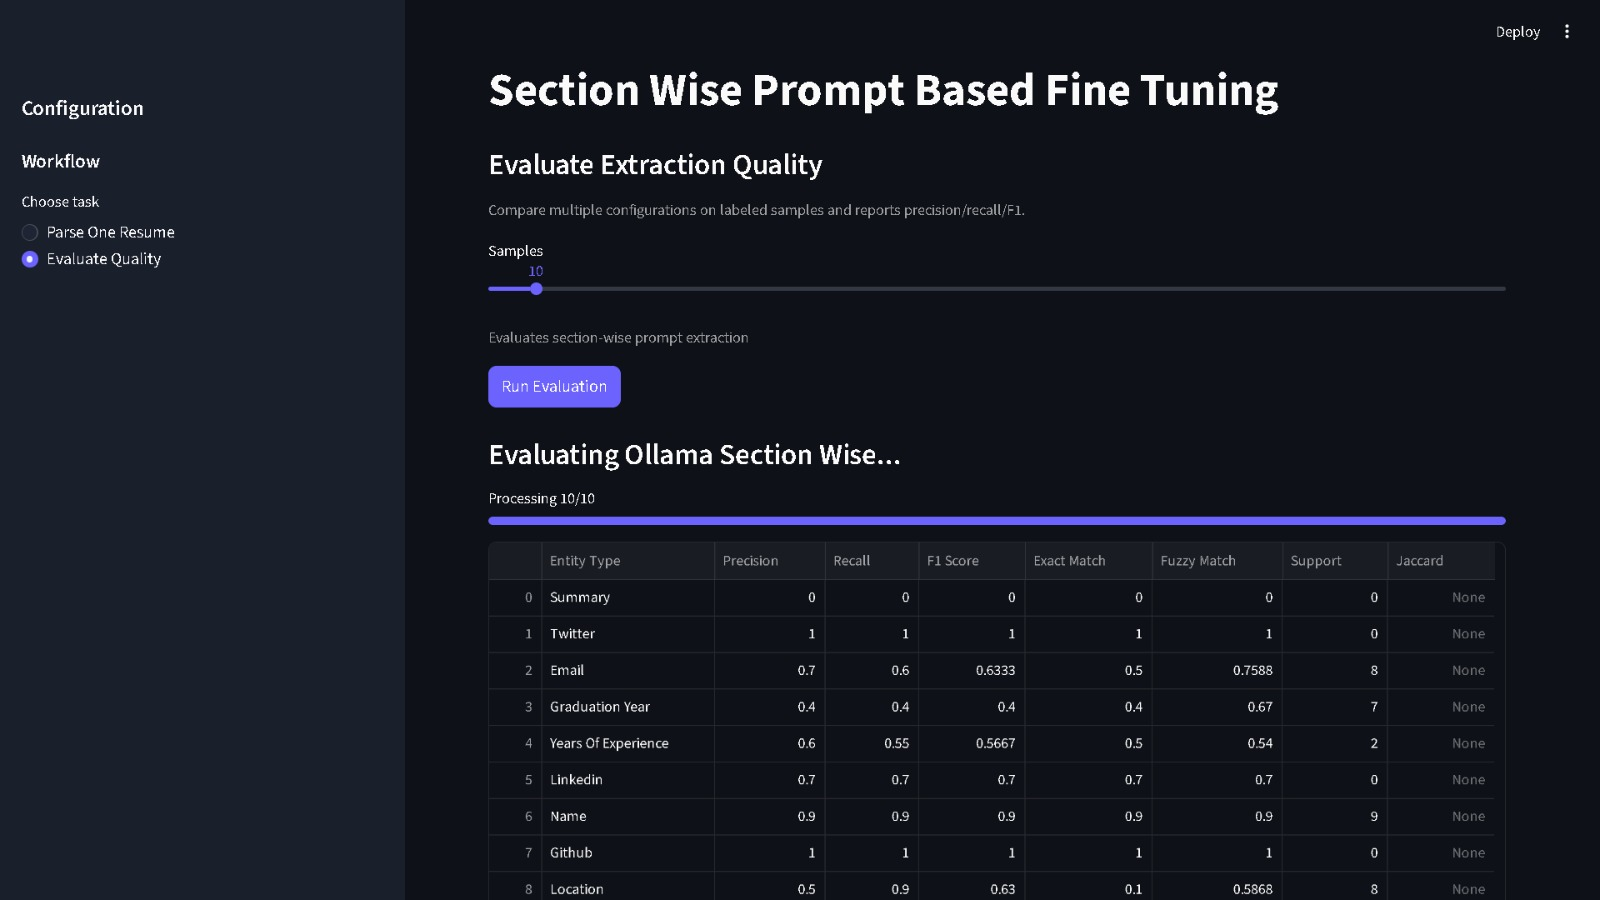
\includegraphics[width=0.9\textwidth]{image18.png}
\\[2pt]
\footnotesize Evaluate Quality: results table
\end{figure}

\vspace{4pt}
\noindent Basic model (ollama-basic) screenshots:

\begin{figure}[H]
\centering
\begin{minipage}{0.48\textwidth}
\centering
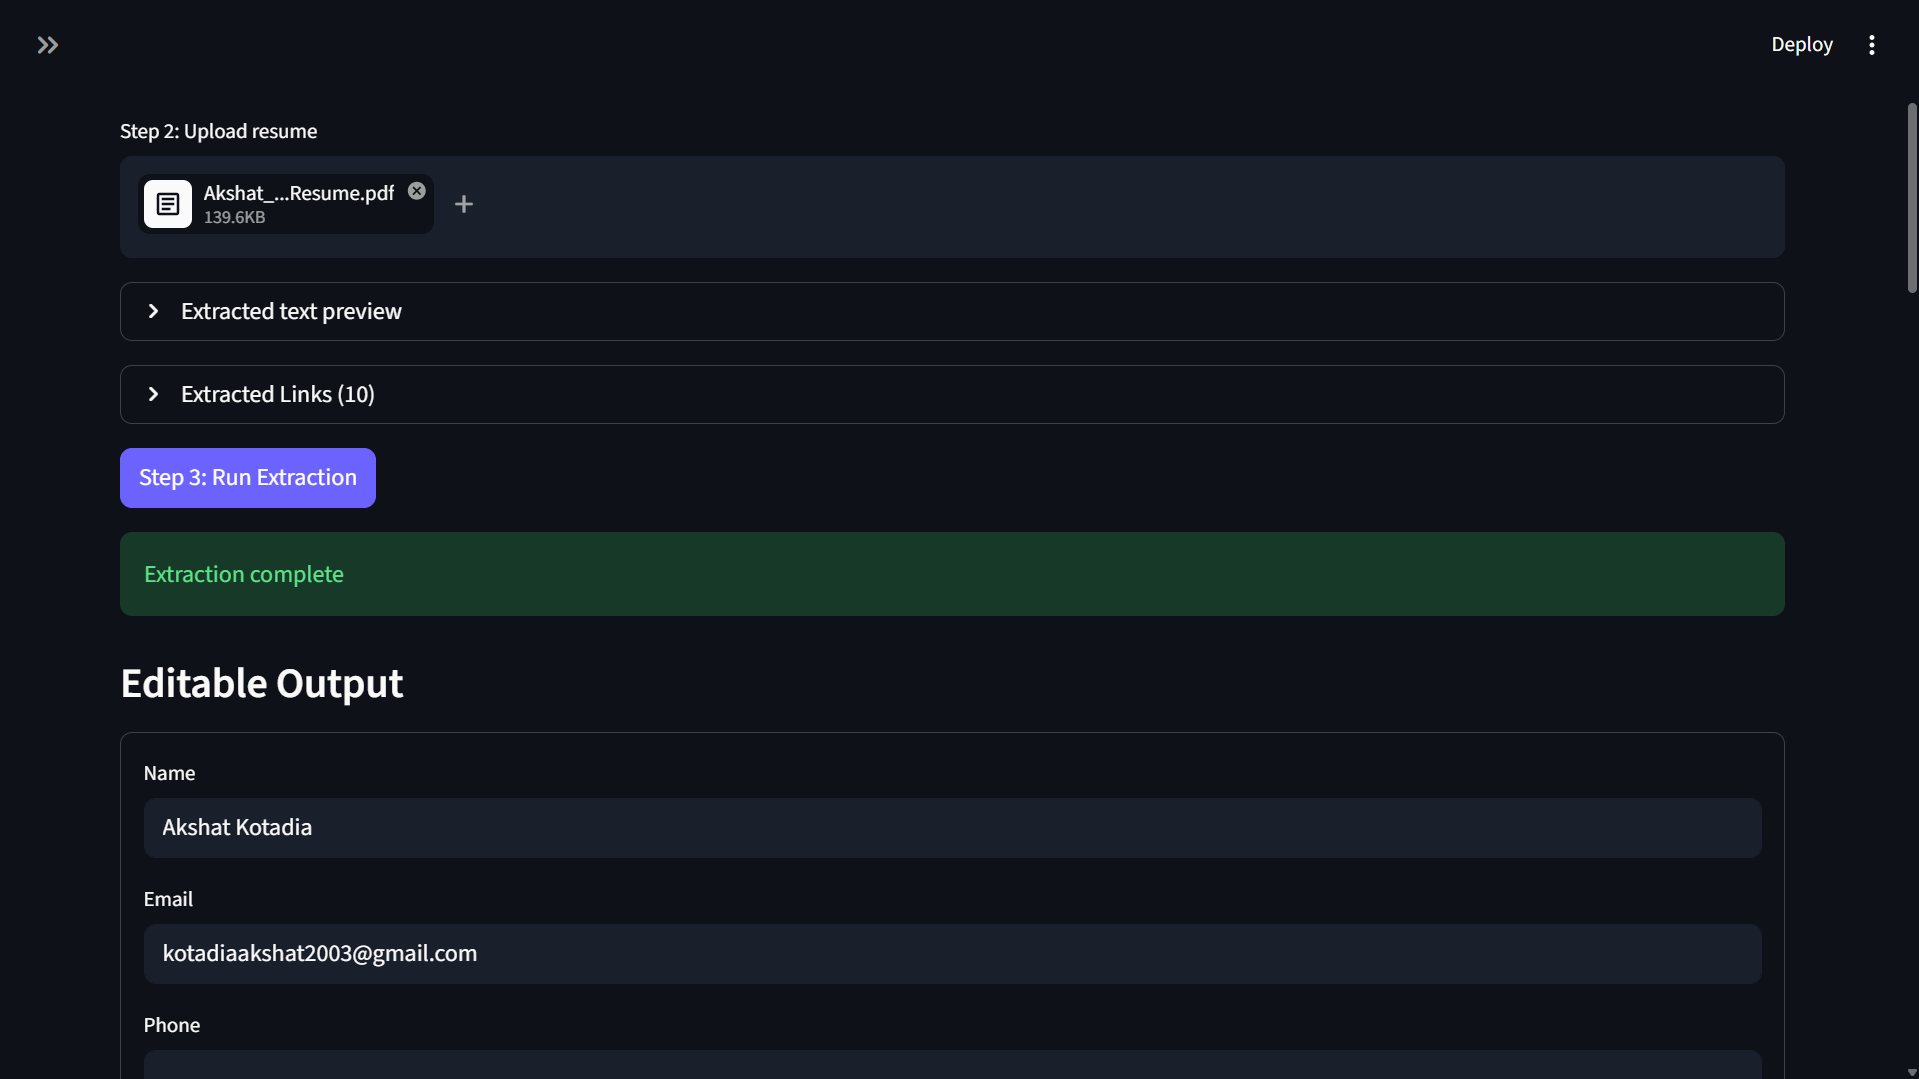
\includegraphics[width=\textwidth]{image19.png}
\\[2pt]
\footnotesize Basic model: upload resume and run extraction
\end{minipage}
\hfill
\begin{minipage}{0.48\textwidth}
\centering
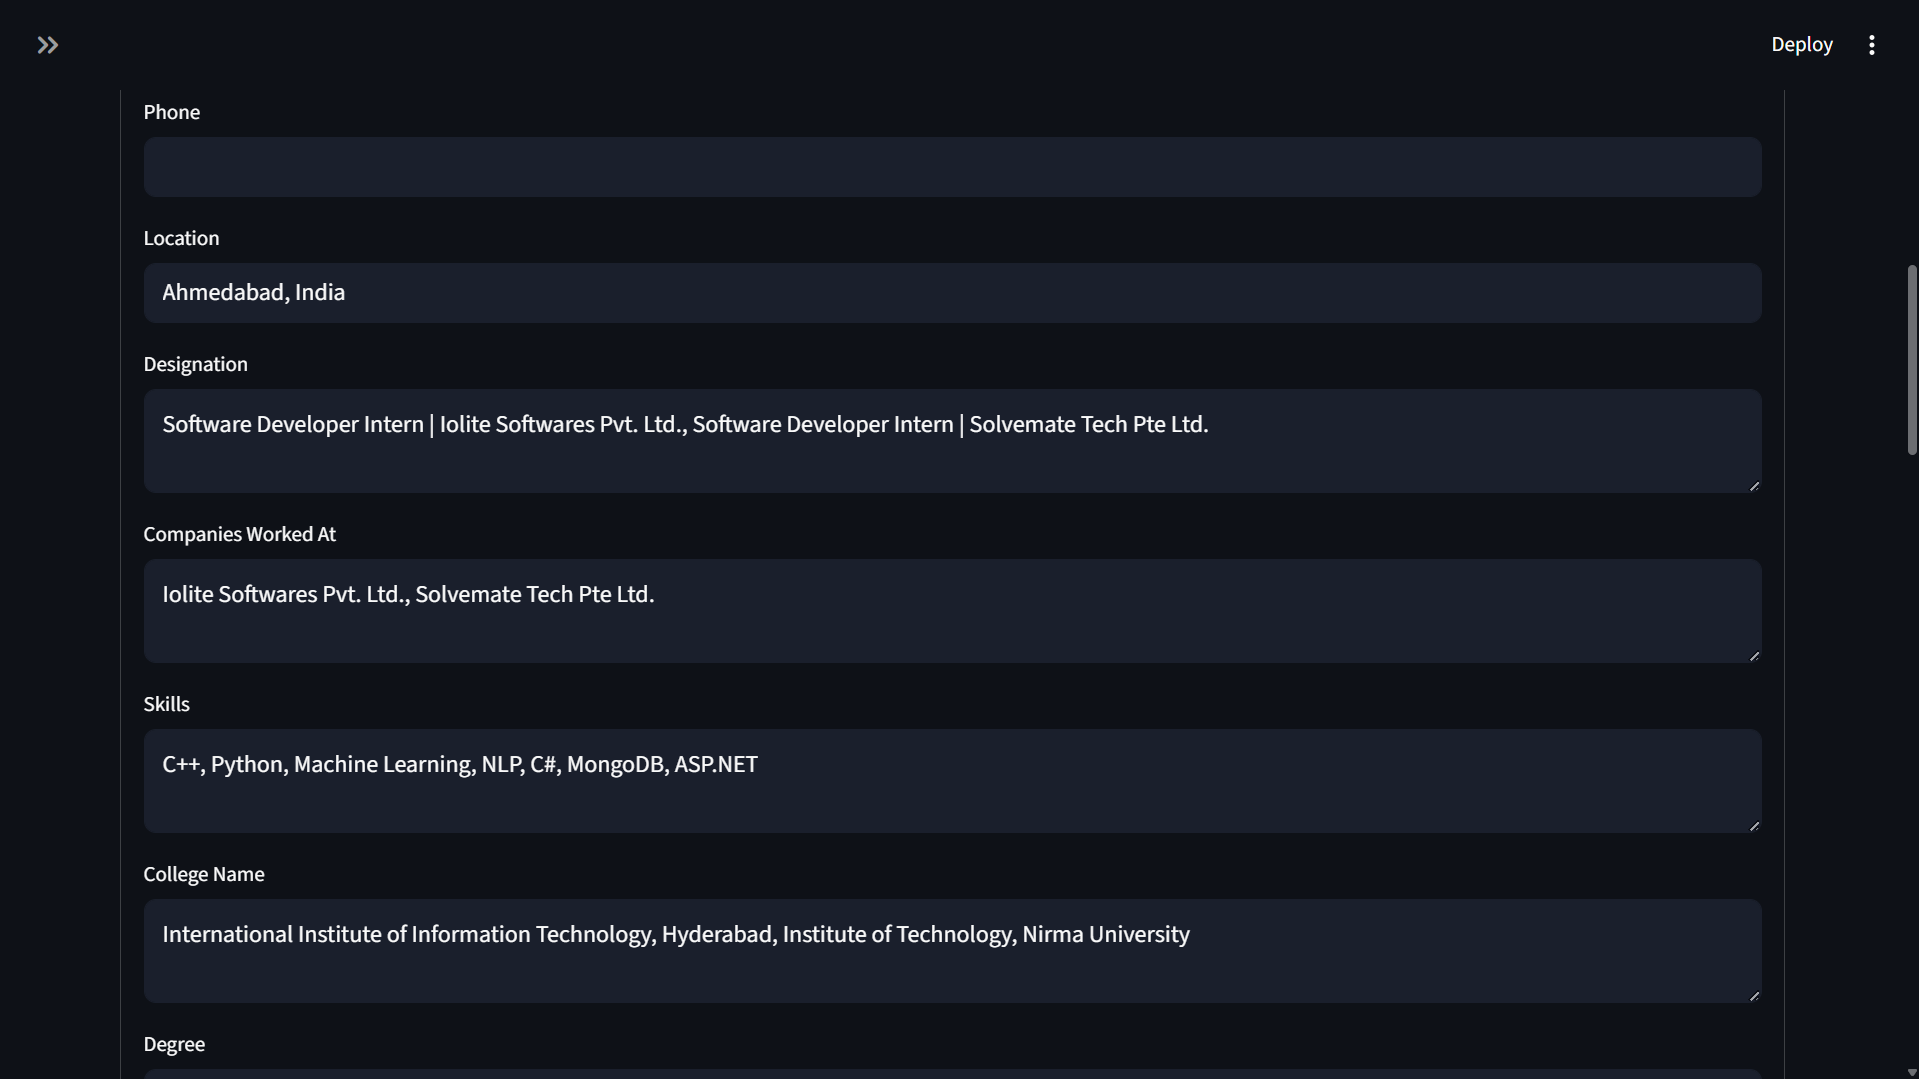
\includegraphics[width=\textwidth]{image20.png}
\\[2pt]
\footnotesize Basic model: editable output (contact, designation, skills)
\end{minipage}
\end{figure}

\begin{figure}[H]
\centering
\begin{minipage}{0.48\textwidth}
\centering
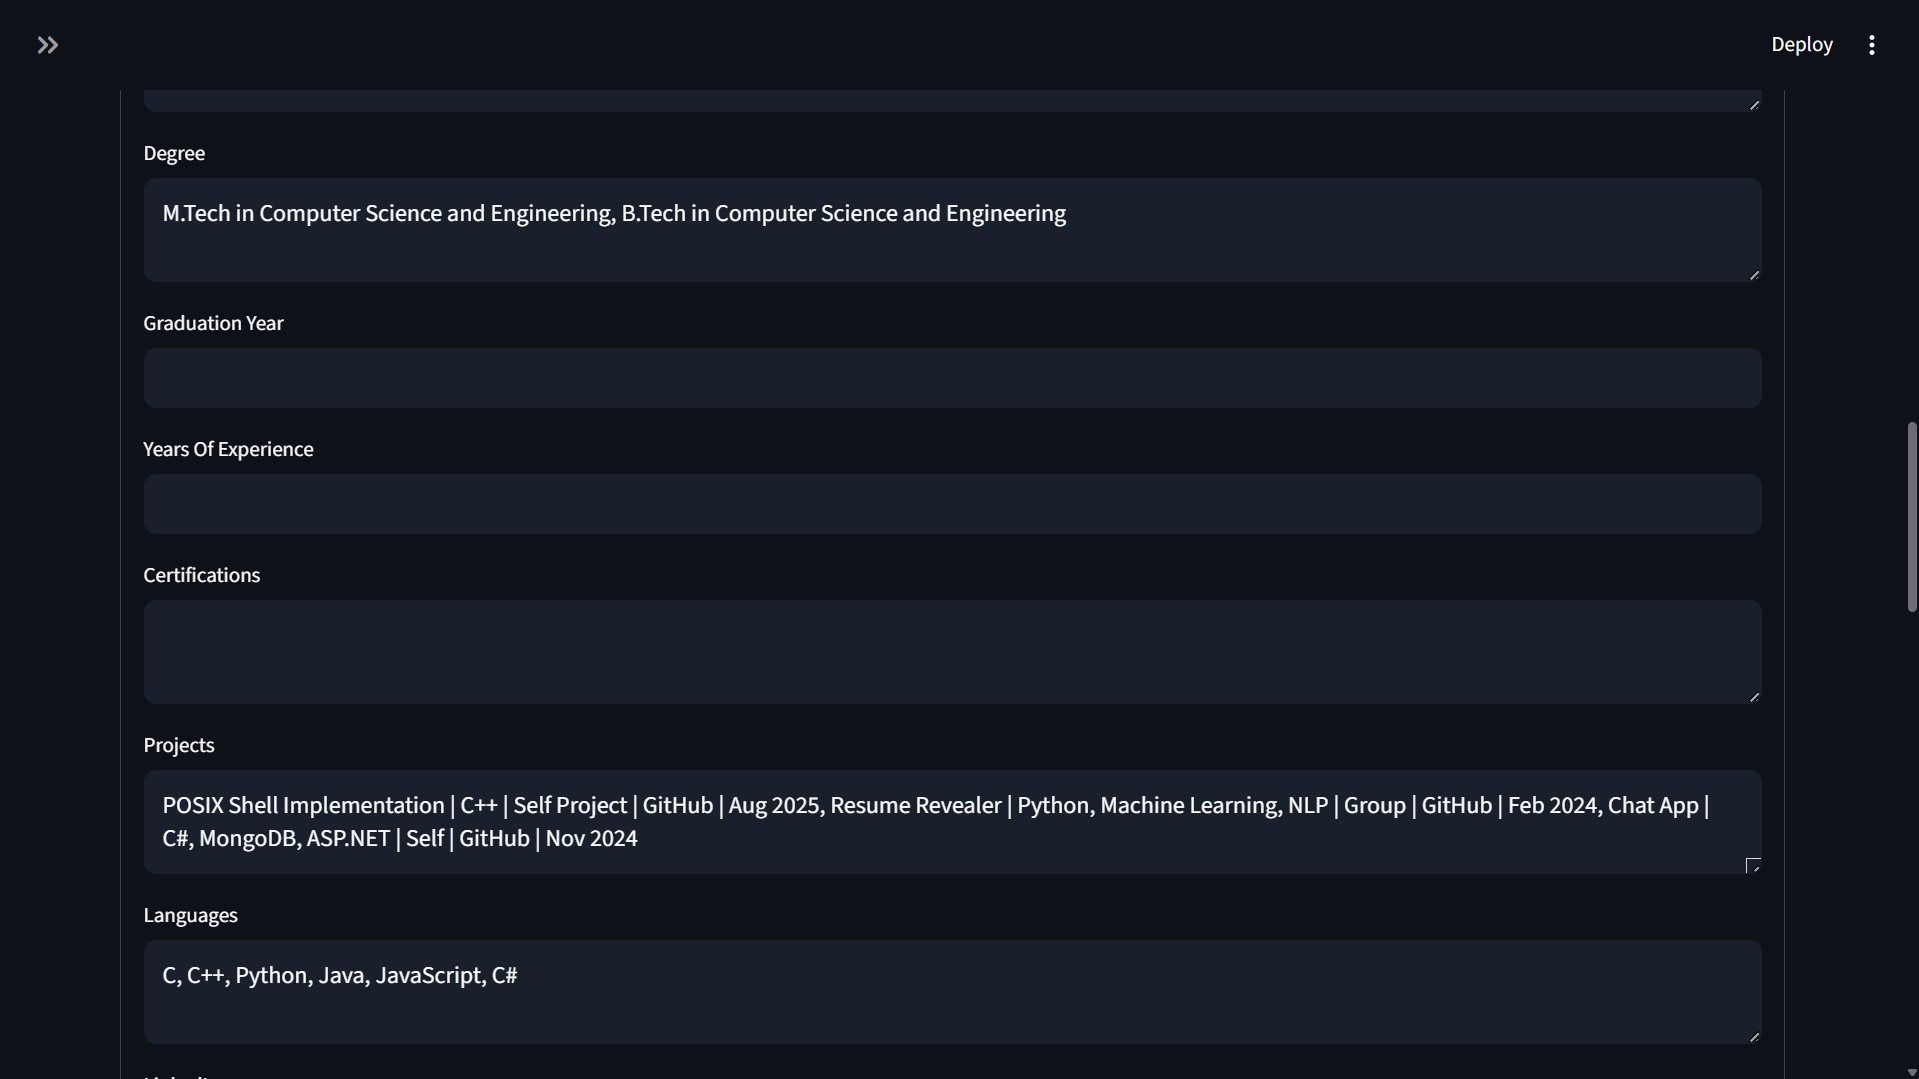
\includegraphics[width=\textwidth]{image21.png}
\\[2pt]
\footnotesize Basic model: editable output (education, projects, languages)
\end{minipage}
\hfill
\begin{minipage}{0.48\textwidth}
\centering
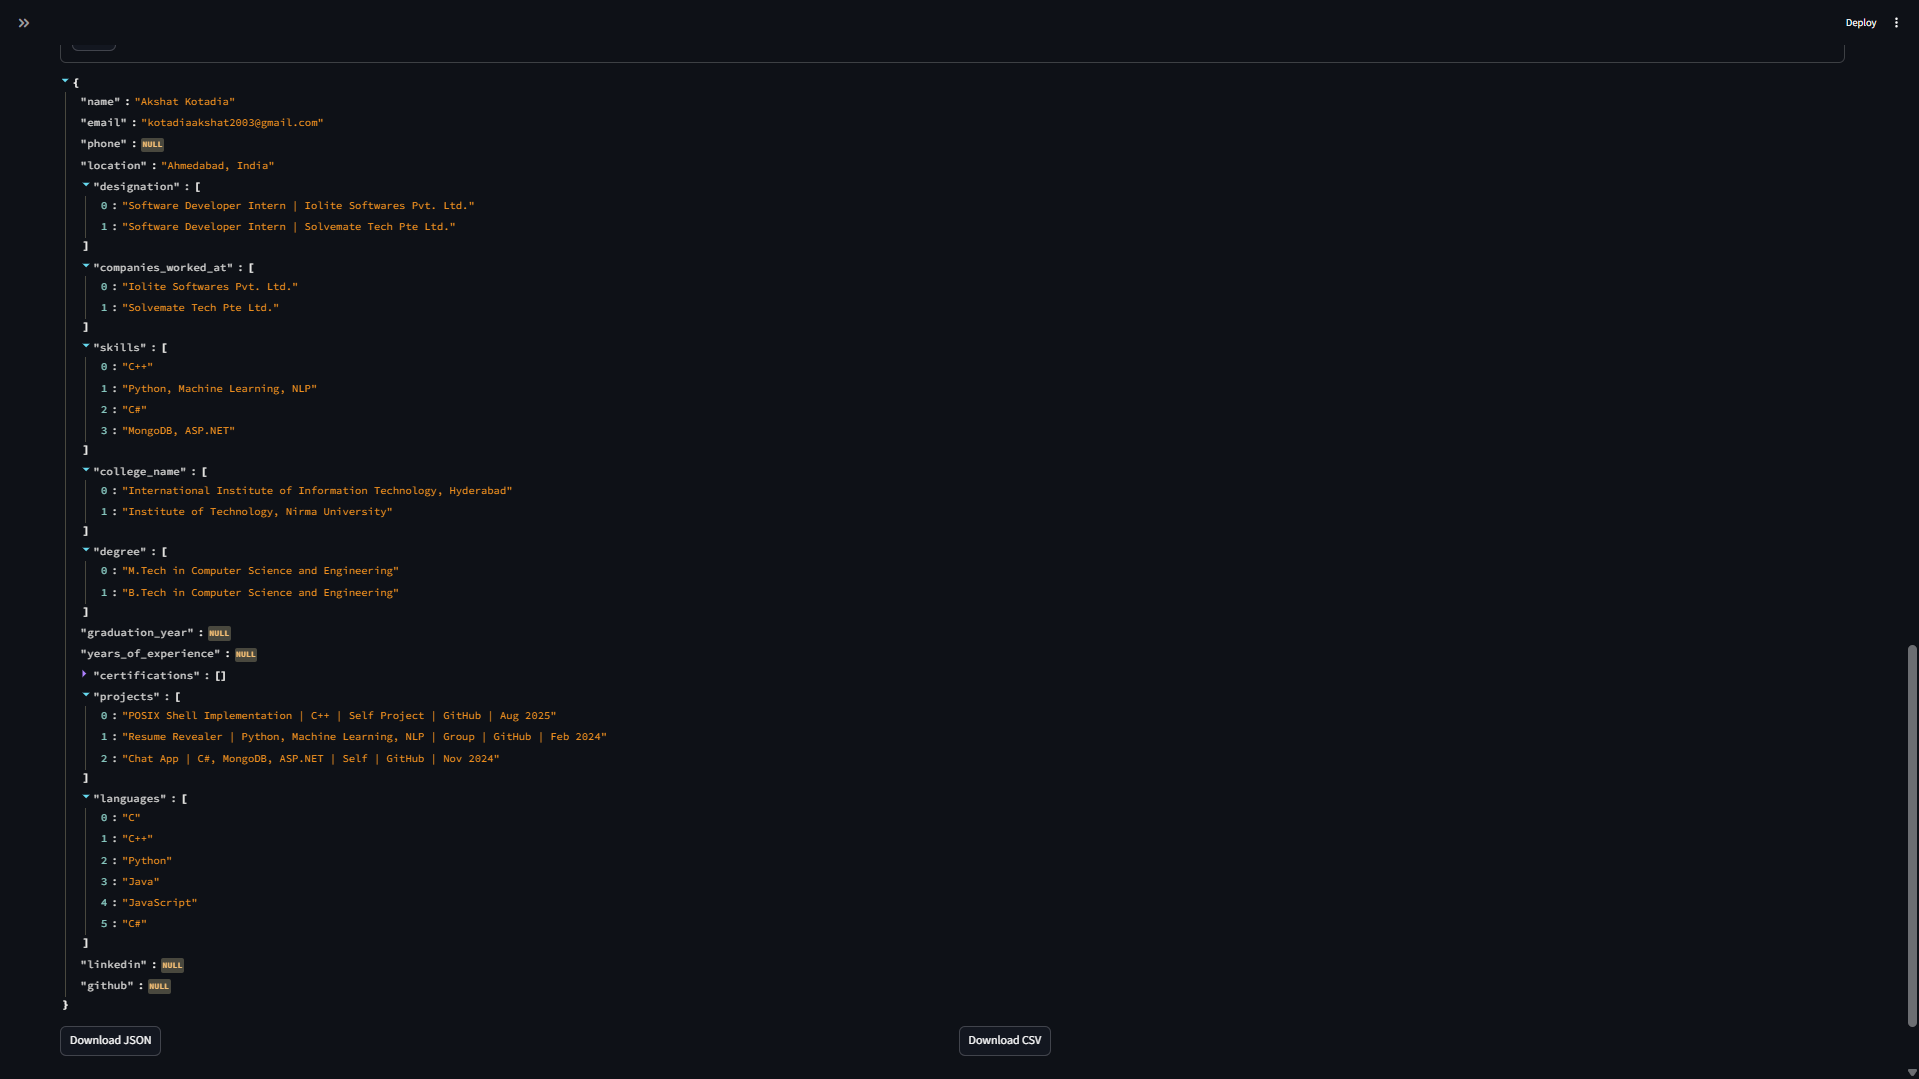
\includegraphics[width=\textwidth]{image22.png}
\\[2pt]
\footnotesize Basic model: final JSON output and downloads
\end{minipage}
\end{figure}

\begin{figure}[H]
\centering
\begin{minipage}{0.48\textwidth}
\centering
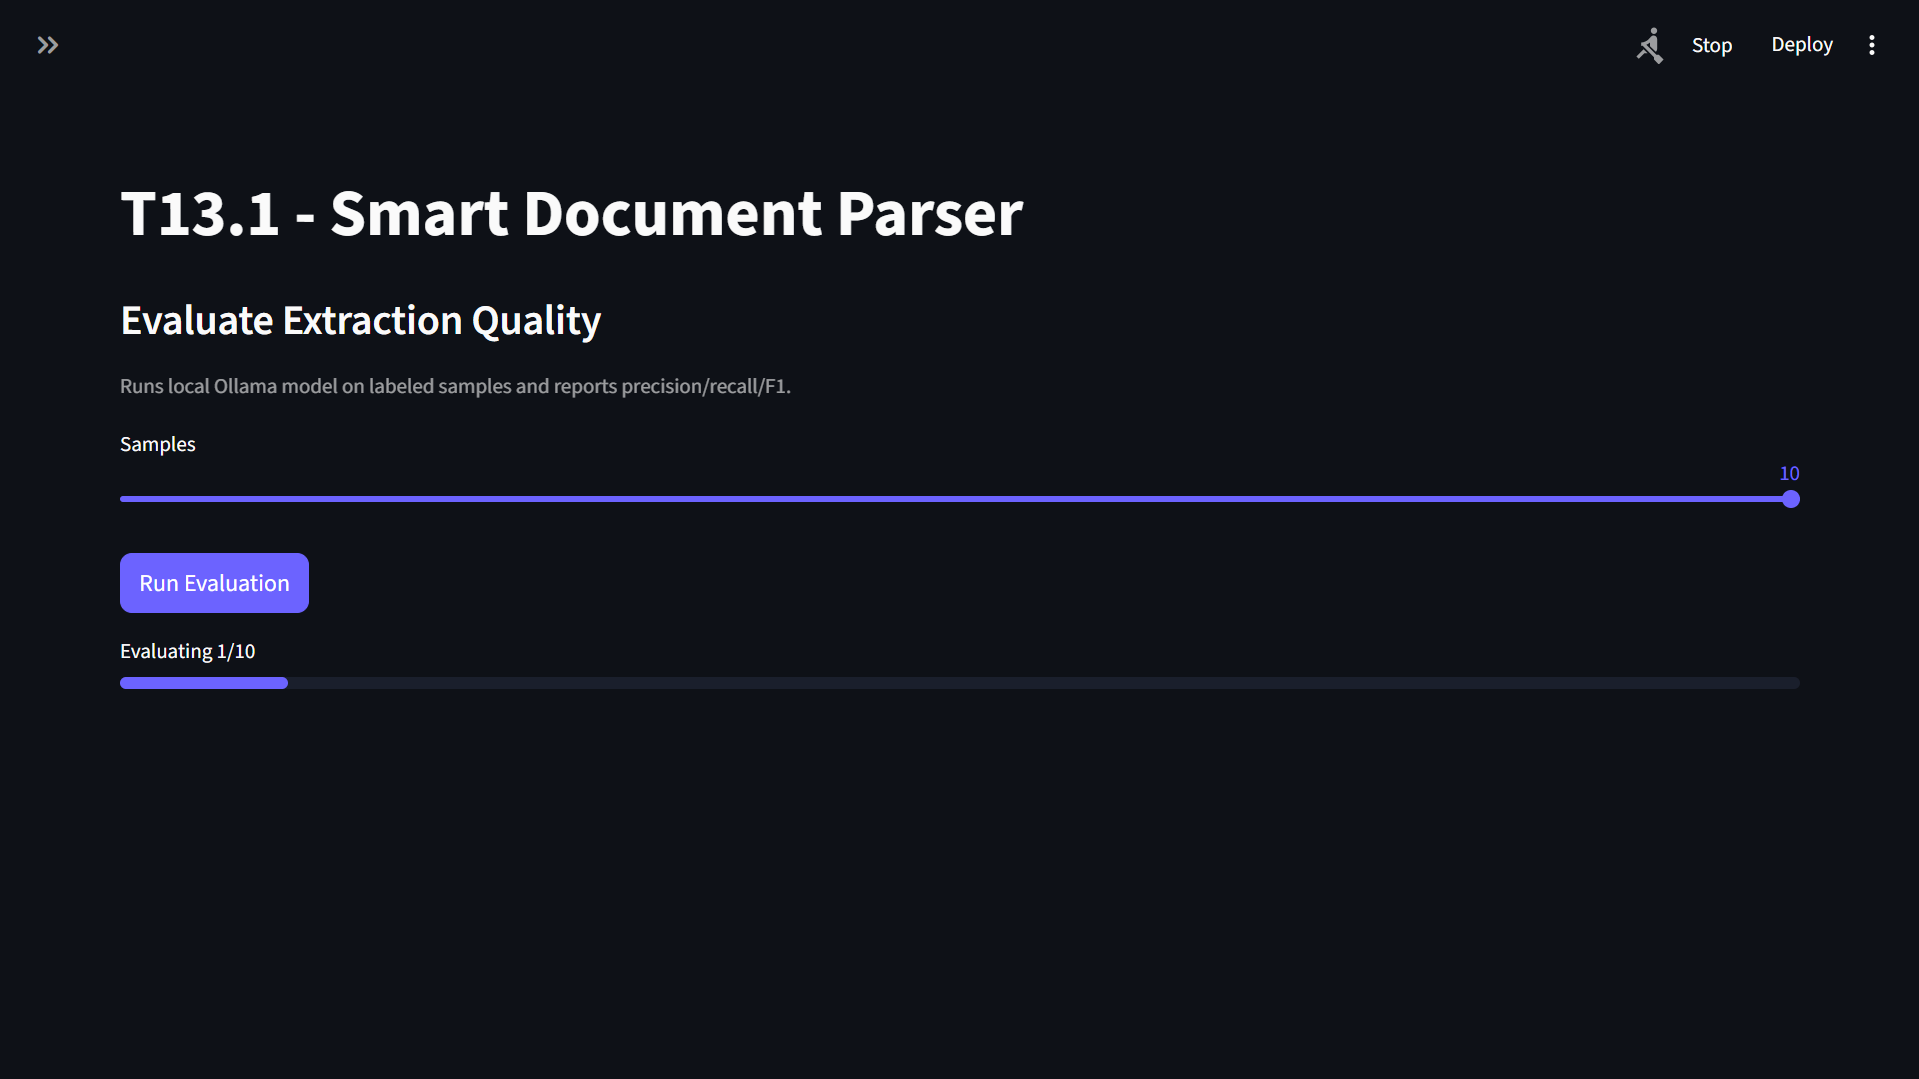
\includegraphics[width=\textwidth]{image23.png}
\\[2pt]
\footnotesize Basic model: evaluation setup and progress
\end{minipage}
\hfill
\begin{minipage}{0.48\textwidth}
\centering
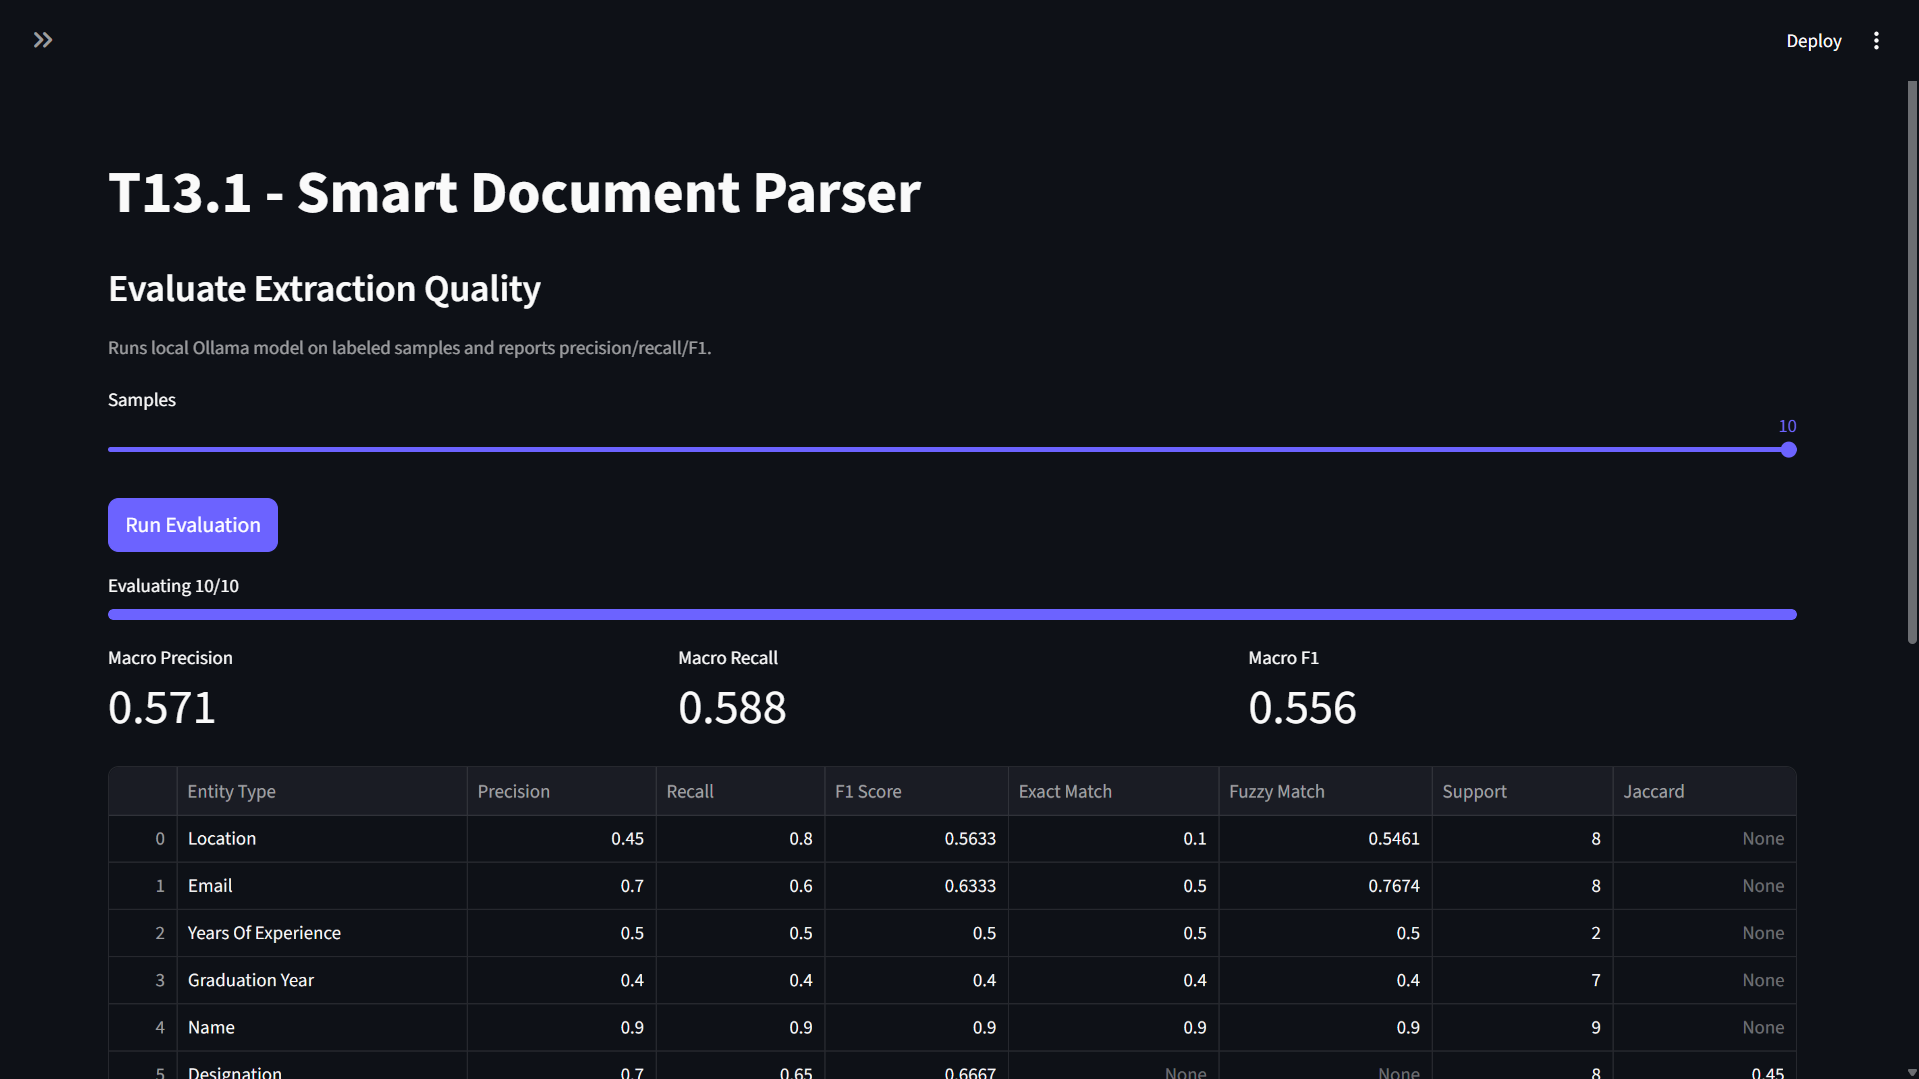
\includegraphics[width=\textwidth]{image24.png}
\\[2pt]
\footnotesize Basic model: evaluation results and metrics table
\end{minipage}
\end{figure}


\begin{thebibliography}{9}
\bibitem{dataset}
Dataturks. Resume Entities for NER. Kaggle, 2019.\newline
\href{https://kaggle.com/datasets/dataturks/resume-entities-for-ner}{https://kaggle.com/datasets/dataturks/resume-entities-for-ner}

\bibitem{streamlit}
Streamlit Team. Streamlit Documentation.\newline
\href{https://docs.streamlit.io}{https://docs.streamlit.io}

\bibitem{ollama}
Ollama Team. Ollama Documentation.\newline
\href{https://ollama.ai}{https://ollama.ai}

\bibitem{llama32}
Meta AI. Llama 3.2 Model Card.\newline
\href{https://ai.meta.com/llama/}{https://ai.meta.com/llama/}

\bibitem{pymupdf}
Artifex Software. PyMuPDF Documentation.\newline
\href{https://pymupdf.readthedocs.io}{https://pymupdf.readthedocs.io}

\bibitem{pydantic}
Samuel Colvin et al. Pydantic Documentation.\newline
\href{https://docs.pydantic.dev}{https://docs.pydantic.dev}

\bibitem{easyocr}
JaidedAI. EasyOCR: Ready-to-Use OCR with Deep Learning. GitHub Repository.\newline
\href{https://github.com/JaidedAI/EasyOCR}{https://github.com/JaidedAI/EasyOCR}
\end{thebibliography}

\end{document}
